% Options for packages loaded elsewhere
\PassOptionsToPackage{unicode}{hyperref}
\PassOptionsToPackage{hyphens}{url}
\documentclass[
  11pt,
]{article}
\usepackage{xcolor}
\usepackage[margin=25mm]{geometry}
\usepackage{amsmath,amssymb}
\setcounter{secnumdepth}{-\maxdimen} % remove section numbering
\usepackage{iftex}
\ifPDFTeX
  \usepackage[T1]{fontenc}
  \usepackage[utf8]{inputenc}
  \usepackage{textcomp} % provide euro and other symbols
\else % if luatex or xetex
  \usepackage{unicode-math} % this also loads fontspec
  \defaultfontfeatures{Scale=MatchLowercase}
  \defaultfontfeatures[\rmfamily]{Ligatures=TeX,Scale=1}
\fi
\usepackage{lmodern}
\ifPDFTeX\else
  % xetex/luatex font selection
\fi
% Use upquote if available, for straight quotes in verbatim environments
\IfFileExists{upquote.sty}{\usepackage{upquote}}{}
\IfFileExists{microtype.sty}{% use microtype if available
  \usepackage[]{microtype}
  \UseMicrotypeSet[protrusion]{basicmath} % disable protrusion for tt fonts
}{}
\makeatletter
\@ifundefined{KOMAClassName}{% if non-KOMA class
  \IfFileExists{parskip.sty}{%
    \usepackage{parskip}
  }{% else
    \setlength{\parindent}{0pt}
    \setlength{\parskip}{6pt plus 2pt minus 1pt}}
}{% if KOMA class
  \KOMAoptions{parskip=half}}
\makeatother
\usepackage{longtable,booktabs,array}
\newcounter{none} % for unnumbered tables
\usepackage{calc} % for calculating minipage widths
% Correct order of tables after \paragraph or \subparagraph
\usepackage{etoolbox}
\makeatletter
\patchcmd\longtable{\par}{\if@noskipsec\mbox{}\fi\par}{}{}
\makeatother
% Allow footnotes in longtable head/foot
\IfFileExists{footnotehyper.sty}{\usepackage{footnotehyper}}{\usepackage{footnote}}
\makesavenoteenv{longtable}
\usepackage{graphicx}
\makeatletter
\newsavebox\pandoc@box
\newcommand*\pandocbounded[1]{% scales image to fit in text height/width
  \sbox\pandoc@box{#1}%
  \Gscale@div\@tempa{\textheight}{\dimexpr\ht\pandoc@box+\dp\pandoc@box\relax}%
  \Gscale@div\@tempb{\linewidth}{\wd\pandoc@box}%
  \ifdim\@tempb\p@<\@tempa\p@\let\@tempa\@tempb\fi% select the smaller of both
  \ifdim\@tempa\p@<\p@\scalebox{\@tempa}{\usebox\pandoc@box}%
  \else\usebox{\pandoc@box}%
  \fi%
}
% Set default figure placement to htbp
\def\fps@figure{htbp}
\makeatother
\setlength{\emergencystretch}{3em} % prevent overfull lines
\providecommand{\tightlist}{%
  \setlength{\itemsep}{0pt}\setlength{\parskip}{0pt}}
\usepackage{bookmark}
\IfFileExists{xurl.sty}{\usepackage{xurl}}{} % add URL line breaks if available
\urlstyle{same}
\hypersetup{
  hidelinks,
  pdfcreator={LaTeX via pandoc}}

\author{}
\date{}

\begin{document}

\section{Ext groups, absorption and Brown--Douglas--Fillmore
theory}\label{ext-groups-absorption-and-browndouglasfillmore-theory}

\emph{Self-checked by the writing AI, GPT-6.1 Sol (OpenAI). Public
domain (CC0).}

An extension can be nontrivial for two different reasons. Its quotient
relation might have a numerical obstruction to lifting, as the shift
does, or the chosen representation might contain extra split summands.
Extension groups retain the first kind of information and discard the
second. This is why adding extensions is followed by a stabilization
relation.

We begin with arbitrary C*-algebras \(A\) and \(B\). Separability of
\(A\) enters the construction of inverses. Section 2 proves the strict
Hilbert-module Stinespring construction, including its adjointability
and minimality assertions. Section 3 proves the equivalence of tensor
nuclearity with finite-matrix approximation, and completely positive
lifting with arbitrary target algebra and ideal. The precise outstanding
dependencies in the planar classification assertions are stated where
they arise.

Throughout, \(J=B\otimes\mathcal K\), \(M=M(J)\), \(Q=M/J\), and
\(q:M\to Q\) is the quotient map. Tensor products here are spatial. All
inner products are conjugate linear in the first variable and linear in
the second, including the scalar inner products in Section 6. For
\(B=\mathbb C\) these are the compact operators, bounded operators, and
Calkin algebra on an infinite-dimensional separable Hilbert space.

\subsection{1. Adding quotient
relations}\label{adding-quotient-relations}

Choose isometries \(s_1,s_2\in M\) satisfying

\[
s_i^*s_j=\delta_{ij}1,\qquad s_1s_1^*+s_2s_2^*=1.
\]

They exist without a countability assumption on \(B\): on
\(\ell^2(\mathbb N_0)\), send the \(n\)-th basis vector to the \(2n\)-th
or the \(2n+1\)-st basis vector, and tensor the resulting operators with
the multiplier identity of \(B\). These operators act adjointably on the
standard module \(H_B=\ell^2(\mathbb N_0,B)\), whose compact algebra is
\(B\otimes\mathcal K\). The identification
\(\mathcal L(H_B)=M(B\otimes\mathcal K)\) is proved in
\href{https://kokunoyumeto.github.io/open-math-courses/courses/KT-CP/prerequisites/hilbert-c-star-modules-and-morita-equivalence/compact-operators-multipliers-and-the-strict-topology.html}{\emph{Compact
operators, multipliers and the strict topology}, Theorem 4.1 and
Exercise 3}. Those results allow arbitrary coefficient algebras.

For Busby maps \(\tau_1,\tau_2:A\to Q\), define

\[
(\tau_1\oplus\tau_2)(a)
=q(s_1)\tau_1(a)q(s_1)^*+q(s_2)\tau_2(a)q(s_2)^*.
\]

Orthogonality makes this a homomorphism. For instance, the cross terms
in the product of the expressions for \(a\) and \(b\) vanish, while the
diagonal terms give \(\tau_i(ab)\).

\subsubsection{Proposition 1.1. Addition of strong equivalence
classes}\label{proposition-1.1.-addition-of-strong-equivalence-classes}

Addition is independent of the chosen isometries up to strong unitary
equivalence. It is associative and commutative on strong equivalence
classes. Split extensions are closed under addition.

\textbf{Proof.} If \(t_1,t_2\) are another pair, set

\[
U=t_1s_1^*+t_2s_2^*.
\]

Then \(U^*U=UU^*=1\) and \(Us_i=t_i\). Conjugation by \(q(U)\)
identifies the two sums. If \(\tau_i'=\operatorname{Ad}(q(U_i))\tau_i\),
the multiplier unitary

\[
W=s_1U_1s_1^*+s_2U_2s_2^*
\]

conjugates the sum of the \(\tau_i\) to the sum of the \(\tau_i'\). Thus
addition is also independent of the strong representatives.

The multiplier unitary \(s_1s_2^*+s_2s_1^*\) exchanges the two summands.
For associativity, the two parenthesizations use the three-isometry
families

\[
(s_1s_1,s_1s_2,s_2),\qquad(s_1,s_2s_1,s_2s_2).
\]

Within each family, the range projections are orthogonal and sum to one.
The sum \(\sum_{i=1}^3t_i r_i^*\) is consequently a unitary intertwining
the two families. It conjugates the two parenthesized Busby maps.

Finally, if \(L_i:A\to M\) are homomorphic lifts, then
\(a\mapsto s_1L_1(a)s_1^*+s_2L_2(a)s_2^*\) is a homomorphic lift of the
sum. \(\square\)

Write \(\mathscr E(A,B)\) for this commutative semigroup. It need not
have an identity represented by the zero Busby map: putting a relation
into a proper corner can change its strong equivalence class. The next
quotient is therefore an actual part of the definition.

Two maps are \textbf{stably strongly equivalent} if there are split
Busby maps \(\sigma_1,\sigma_2\) such that

\[
\tau_1\oplus\sigma_1\sim_s\tau_2\oplus\sigma_2.
\]

We define \(\operatorname{Ext}(A,B)\) to be the quotient by this
relation. We also write
\(\operatorname{Ext}(A)=\operatorname{Ext}(A,\mathbb C)\).

\subsubsection{Proposition 1.2. The stabilized semigroup has
zero}\label{proposition-1.2.-the-stabilized-semigroup-has-zero}

Stable strong equivalence is an equivalence relation compatible with
addition. Its quotient is an abelian monoid. All split maps represent
its zero element, and the class of \(\tau\oplus0\) equals the class of
\(\tau\).

\textbf{Proof.} Reflexivity follows by adding a zero map to both sides.
Symmetry is immediate. For transitivity, add the split summands in the
two given equivalences and use associativity and commutativity. For
example, if \(x+t_1=y+t_2\) and \(y+t_3=z+t_4\) in \(\mathscr E(A,B)\),
then

\[
x+(t_1+t_3)=z+(t_4+t_2).
\]

The new summands are split. Adding another extension to a stable
equivalence preserves it; hence addition descends.

For a split class \(t\), commutativity gives \(t+0=0+t\), so \(t\) and
\(0\) become equivalent. For any \(x\), associativity gives

\[
(x+0)+0=x+(0+0).
\]

Since both \(0\) and \(0+0\) are split, \(x+0\) and \(x\) become
equivalent. The common class of split extensions is therefore an
identity. \(\square\)

The distinction between strong equivalence and stable strong equivalence
prevents a common mistake: a unital Busby map need not be strongly
equivalent to its sum with the zero map. Their images of \(1\) have
different support projections. They do represent the same element of
\(\operatorname{Ext}\).

\subsubsection{Proposition 1.3. Corona conjugacies after
stabilization}\label{proposition-1.3.-corona-conjugacies-after-stabilization}

Using weak unitary equivalence instead of strong unitary equivalence
gives the same ordinary \(\operatorname{Ext}(A,B)\).

\textbf{Proof.} Suppose \(\tau_2=\operatorname{Ad}(v)\tau_1\) for a
unitary \(v\in Q\). The unitary \(\operatorname{diag}(v,v^*)\in M_2(Q)\)
lifts to a multiplier unitary. To prove this lifting assertion, the path

\[
\operatorname{diag}(v,1)R_t\operatorname{diag}(1,v^*)R_t^*,
\qquad
R_t=\begin{pmatrix}\cos t&-\sin t\\\sin t&\cos t\end{pmatrix},
\quad0\leq t\leq\pi/2,
\]

runs from \(\operatorname{diag}(v,v^*)\) to \(1\). Every unitary
connected to \(1\) in a quotient lifts to a unitary: partition a path
from \(1\) into finitely many increments sufficiently close to \(1\) to
have a continuous self-adjoint logarithm. Lift each logarithm
self-adjointly and multiply its exponential by the previous lift. This
gives exactly the endpoint unitary, with no limiting approximation
needed.

Conjugation by the resulting lift takes
\(\operatorname{diag}(\tau_1,0)\) to \(\operatorname{diag}(\tau_2,0)\).
Thus adding the split zero extension changes a weak equivalence into a
strong one. Apply this to the weak equivalence witnessing any stable
relation, and use Proposition 1.2 to discard the extra zero maps. The
converse is immediate. \(\square\)

The proof uses zero summands. It does not assert the analogous equality
for a stabilization relation that requires every added extension to have
a unital lift.

\subsection{2. Why a completely positive lift produces an
inverse}\label{why-a-completely-positive-lift-produces-an-inverse}

A completely positive lift can be placed in a corner of a homomorphism.
The other corner will be the inverse. We first make the needed
stabilization precise, including the case in which \(B\) is not
\(\sigma\)-unital.

Recall that \(\mathcal L(E,F)\) denotes the adjointable maps between
Hilbert \(B\)-modules. A unitary between modules is a surjective
\(B\)-linear inner-product-preserving map; its inverse is its adjoint.

\subsubsection{Lemma 2.0a. The strict KSGNS
construction}\label{lemma-2.0a.-the-strict-ksgns-construction}

Let \(C,B\) be arbitrary C*-algebras, let \(H\) be a Hilbert
\(B\)-module, and let \(\psi:C\to\mathcal L(H)\) be completely positive.
Suppose a positive contractive approximate identity \((e_\lambda)\)
satisfies \(\psi(e_\lambda)\to h\) strictly. Then there are a Hilbert
\(B\)-module \(E\), a nondegenerate homomorphism
\(\pi:C\to\mathcal L(E)\), and an adjointable map \(V:H\to E\), with

\[
\psi(c)=V^*\pi(c)V,\qquad V^*V=h,\qquad
E=\overline{\operatorname{span}}\pi(C)VH.
\]

This dilation is unique up to a unitary intertwining \(\pi\) and \(V\).
Moreover \(\|V\|^2=\|\psi\|\). If \(h=1\), the range of \(V\) is
complemented. No separability or \(\sigma\)-unitality assumption is
required.

\textbf{Proof.} Complete positivity implies positivity and boundedness;
the boundedness assertion is proved in
\href{https://kokunoyumeto.github.io/open-math-courses/courses/foundations-of-von-neumann-algebras/completely-positive-maps.html}{\emph{Completely
positive maps}, Proposition 3.2}. On \(C\odot H\), define

\[
\left\langle\sum_i c_i\otimes x_i,\sum_j d_j\otimes y_j\right\rangle
=\sum_{i,j}\langle x_i,\psi(c_i^*d_j)y_j\rangle_B.
\]

The matrix \([c_i^*c_j]\) is positive, being a row's Gram matrix. Its
image \([\psi(c_i^*c_j)]\) is positive in \(\mathcal L(H^n)\); its
quadratic form on the column \((x_i)\) is the displayed squared length.
Thus the form is positive semidefinite. The module Cauchy--Schwarz
inequality makes its null vectors orthogonal to every vector and its
null space a right submodule. Quotient and complete to obtain \(E\).
These operations, including the coefficient-order Cauchy--Schwarz
inequality and the semidefinite quotient and completion, are proved in
\href{supporting/hilbert-c-star-modules-and-morita-equivalence/hilbert-module-foundations.html\#mf-002}{Ordinary
Hilbert C*-module foundations, MF.2--MF.3}.

Left multiplication gives \(\pi(c)[d\otimes x]=[cd\otimes x]\). For
\(z=\sum_i d_i\otimes x_i\), positivity of

\[
[d_i^*(\|c\|^2 1-c^*c)d_j]
\]

in the unitization, followed by complete positivity, gives
\(\langle\pi(c)z,\pi(c)z\rangle\leq\|c\|^2\langle z,z\rangle\).
Consequently left multiplication preserves null vectors and extends
boundedly. Its adjoint is left multiplication by \(c^*\), directly from
the form. It is multiplicative. Also
\(\pi(e_\lambda)[d\otimes x]\to[d\otimes x]\), since
\(e_\lambda d\to d\). The bound
\(\|[d\otimes x]\|\leq\|\psi\|^{1/2}\|d\|\|x\|\) extends this
convergence to all of \(E\), proving nondegeneracy.

It remains to construct an adjointable \(V\); an arbitrary bounded
module map would not suffice. Strict convergence here means convergence
of \(\psi(e_\lambda)x\) and its adjoint action on every \(x\in H\). This
characterization on bounded sets is
\href{https://kokunoyumeto.github.io/open-math-courses/courses/KT-CP/prerequisites/hilbert-c-star-modules-and-morita-equivalence/compact-operators-multipliers-and-the-strict-topology.html}{\emph{Compact
operators, multipliers and the strict topology}, Proposition 5.1}.

For every positive contraction \(c\in C\),
\(0\leq e_\lambda c e_\lambda\leq e_\lambda^2\leq e_\lambda\). Take
quadratic forms, apply \(\psi\), and pass to the norm limit on each
vector. It follows that \(h\geq\psi(c)\geq0\). The quadratic-form test
for positivity is proved in
\href{supporting/hilbert-c-star-modules-and-morita-equivalence/hilbert-module-foundations.html\#mf-005}{Ordinary
Hilbert C*-module foundations, MF.5}, equation (MF.14).

The map \(\Psi:C^+\to\mathcal L(H)\), \(\Psi(c+t1)=\psi(c)+th\), is
positive. Indeed, positivity of \(c+t1\) implies \(t\geq0\), \(c=c^*\),
and \(\|c_-\|\leq t\). For \(t>0\), the preceding order bound gives
\(\psi(c_-)\leq th\); hence \(\Psi(c+t1)=\psi(c_+)+th-\psi(c_-)\geq0\).
The case \(t=0\) is immediate. Only positivity, rather than complete
positivity, of this auxiliary map is needed.

Put \(p=1-e_\lambda\) and \(r=1-e_\mu\). Both are positive contractions.
Without assuming that they commute,

\[
(e_\lambda-e_\mu)^2=(p-r)^2
\leq2(p^2+r^2)\leq2(p+r).
\]

Applying \(\Psi\) gives

\[
\|[e_\lambda\otimes x]-[e_\mu\otimes x]\|^2
\leq2\|\langle x,(2h-\psi(e_\lambda)-\psi(e_\mu))x\rangle\|
\longrightarrow0.
\]

Thus \(Vx=\lim_\lambda[e_\lambda\otimes x]\) exists, is \(B\)-linear,
and has norm at most \(\|\psi\|^{1/2}\). For a finite tensor sum
\(z=\sum_i[c_i\otimes y_i]\),

\[
\langle Vx,z\rangle=\left\langle x,\sum_i\psi(c_i)y_i\right\rangle.
\]

For any module vector \(w\),
\(\|w\|=\sup_{\|x\|\leq1}\|\langle x,w\rangle\|\): Cauchy--Schwarz
proves the upper bound, and \(x=w/\|w\|\) proves the reverse bound. The
preceding equality therefore makes \(z\mapsto\sum_i\psi(c_i)y_i\) well
defined on the null quotient and bounded by \(\|V\|\|z\|\). Its
extension is exactly \(V^*\). This proves adjointability, including
convergence of the adjoint formula.

Now \(\pi(c)Vx=[c\otimes x]\), by \(ce_\lambda\to c\), so
\(V^*\pi(c)V=\psi(c)\) and minimality follows. Taking limits in
\(V^*[e_\lambda\otimes x]=\psi(e_\lambda)x\) proves \(V^*V=h\).
Compression gives \(\|\psi\|\leq\|V\|^2\), while the construction gave
the reverse inequality. If \(h=1\), \(VV^*\) is the orthogonal
projection onto \(VH\).

For another minimal dilation \((E',\rho,W)\), send
\(\sum_i\pi(c_i)Vx_i\) to \(\sum_i\rho(c_i)Wx_i\). The squared lengths
and mixed inner products coincide by the kernel formula. The map extends
to a surjective inner-product-preserving map, hence a unitary. It
intertwines the representations. Nondegeneracy of both representations
and passage to the approximate-identity limit show that it sends \(V\)
to \(W\); density proves uniqueness. Finally every other positive
contractive approximate identity \((f_\nu)\) satisfies
\(\pi(f_\nu)\to1\) pointwise on \(E\), so
\(\psi(f_\nu)=V^*\pi(f_\nu)V\to V^*V\) strictly. This also verifies
independence of the approximate identity in the definition of
strictness. \(\square\)

\subsubsection{Lemma 2.0b. The ordinary tensor
foundations}\label{lemma-2.0b.-the-ordinary-tensor-foundations}

For arbitrary C*-algebras \(C,D\), the spatial tensor norm is
independent of the faithful Hilbert-space representations used to define
it. It preserves inclusions, and is the smallest C*-norm on
\(C\odot D\). Every C*-norm \(\gamma\) on that algebra satisfies \[
\|z\|_{\min}\leq\gamma(z)\leq\|z\|_{\max},\qquad
\gamma(c\otimes d)=\|c\|\|d\|.
\] There is a unique C*-norm on \(M_n\odot D=M_n(D)\). Tensoring
homomorphisms is contractive for the minimal norm; the flip and
rebracketing are isometric. None of these assertions assumes
separability, units or nuclearity.

\textbf{Proof: construction and independence.} On the algebraic
Hilbert-space tensor product use the product inner product, linear in
its second variable. A finite sum can be written
\(\sum_j e_j\otimes\eta_j\) with the \(e_j\) orthonormal, and its
squared norm is \(\sum_j\|\eta_j\|^2\); this proves positive
definiteness. Completion gives \(H\otimes K\). Expansion in orthonormal
bases of the finite spans of the entries proves that \(T\otimes1\) and
\(1\otimes S\) have norms at most \(\|T\|\) and \(\|S\|\). Their product
has adjoint \(T^*\otimes S^*\), and product unit vectors approaching
both operator norms prove \(\|T\otimes S\|=\|T\|\|S\|\). Flip and
rebracketing preserve the inner products and extend to unitaries.

We spell out the representation facts used here. For a nonzero positive
\(x\) in a unital C*-algebra, evaluation at \(\|x\|\) on \(C^*(1,x)\),
followed by norm-preserving Hahn--Banach extension, gives a functional
\(f\) with \(\|f\|=f(1)=1\) and \(f(x)=\|x\|\). This functional is
positive. Indeed, the first-order expansion of \(f(e^{ith})\) and
\(|f(e^{ith})|\leq1\), for both signs of real \(t\), makes \(f(h)\) real
for self-adjoint \(h\). For \(0\leq h\leq1\),
\(|1-f(h)|\leq\|1-h\|\leq1\) then gives \(f(h)\geq0\). Scaling proves
positivity. The same argument shows that every norm-preserving extension
of a state from a unital subalgebra is a state.

For a state \(f\), the form \(f(x^*y)\) is positive semidefinite.
Applying positivity to \((x+ty)^*(x+ty)\) for complex \(t\) gives
Cauchy--Schwarz, so null vectors are orthogonal to everything. In the
quotient and its completion, left multiplication by \(a\) is bounded
because \[
f(x^*a^*ax)\leq\|a\|^2 f(x^*x),
\] and has adjoint left multiplication by \(a^*\). The class of \(1\) is
cyclic. The direct sum over states is faithful, by the norm-attaining
states just constructed. For a nonunital algebra use its unitization and
restrict to the nondegenerate part; the restriction remains faithful. We
use the earlier functional calculus, positive-square-root and
adjointable-operator proofs specified in the internal dependency
paragraph, rather than an additional representation theorem.

Define \[
\|z\|_{\min}=\sup_{\pi,\rho}\|(\pi\odot\rho)(z)\|,
\qquad z\in C\odot D,
\] over Hilbert-space representations. This is finite, since for
\(z=\sum_i c_i\otimes d_i\) it is at most \(\sum_i\|c_i\|\|d_i\|\). It
is submultiplicative, respects adjoints, and
\(\|z^*z\|_{\min}=\sup_{\pi,\rho}\|(\pi\odot\rho)(z)\|^2=\|z\|_{\min}^2\).
For a faithful pair its product representation is algebraically
injective: vector functionals separate operators, hence their
restrictions span the dual of every finite-dimensional operator
subspace. Applying products of these functionals to a zero image
recovers all algebraic tensor coefficients. Thus the supremum is a norm.

Fix faithful nondegenerate representations \(\pi,\rho\). In the unital
case they are unital. The convex hull of unit vector states of a
faithful representation is weak-* dense in the state space: a separating
continuous real functional would be evaluation at a self-adjoint \(h\),
and would give a state \(f\) with \[
f(h)>\sup_{\|\xi\|=1}\langle\xi,\pi(h)\xi\rangle.
\] Faithfulness preserves spectrum and order, so the supremum on the
right is the maximal spectral value of \(h\), which bounds every state's
value. This is a contradiction. Continuous real weak-* functionals are
finite combinations of evaluations, justifying the asserted form of the
separator.

Put \(r=\|(\pi\odot\rho)(z)\|\). For every \(w\in C\odot D\), the
represented operator inequality gives \[
(f_\xi\otimes g_\eta)(w^*z^*zw)
\leq r^2(f_\xi\otimes g_\eta)(w^*w).
\] Convex combinations and weak-* approximation extend this to every
pair of states \(f,g\), since each expression is a finite sum of
products of evaluations. In their product GNS representation the vectors
\(w(\xi_f\otimes\xi_g)\) are dense, and this inequality bounds the
represented \(z\) by \(r\). Every nondegenerate representation is a
direct sum of cyclic representations: take a maximal orthogonal family
of cyclic reducing subspaces; a nonzero reducing complement would supply
another one. Each cyclic representation is its vector state's GNS
representation, by the map \([a]\mapsto\pi(a)\xi\). Tensor products of
these orthogonal sums are the corresponding sums of cyclic product
representations. Hence every pair has norm at most \(r\), proving
independence.

For nonunital factors, a faithful nondegenerate representation extends
faithfully to the usual unitization: \(\pi(c)+\lambda I=0\), with
\(\lambda\ne0\), would make \(-c/\lambda\) an identity of the original
algebra. If the algebra already has an identity, retain that identity in
this step. Discard zero representation parts before extending other
representations. The unital proof then proves independence on the
original algebraic tensor product. Composing representations with
homomorphisms proves tensor contractivity. Restricting faithful
representations of larger algebras to the nondegenerate parts of
subalgebras preserves faithfulness, and proves tensor inclusions
isometric. The Hilbert-space flip and rebracketing give the remaining
isometries.

\textbf{Proof: the smallest norm for unital factors.} We first justify
the pure-state argument completely. The state space is a weak-* compact
convex subset of the dual unit ball: it is closed, by its defining
positivity and identity conditions, and compact by Banach--Alaoglu. For
positive \(x\), the states taking the maximal value \(\|x\|\) form a
nonempty compact face. A decreasing chain of nonempty compact faces has
nonempty intersection. Zorn's lemma gives a minimal such face. If it
contained two distinct states, a self-adjoint element separating them
would have a proper nonempty maximizing face inside it, a contradiction.
The minimal face is a singleton, hence a pure state. Pure states
therefore norm positive elements, and the direct sum of their GNS
representations is faithful.

If \(f\) is pure and \(0\leq\ell\leq f\), write \(t=\ell(1)\). For
\(0<t<1\), the expression \(f=t(\ell/t)+(1-t)((f-\ell)/(1-t))\) and
extremality give \(\ell=tf\); the cases \(t=0,1\) follow from positivity
and its norm formula. In the GNS representation of \(f\), a positive
contraction \(T\) in the commutant defines
\(\ell(a)=\langle\xi,T\pi(a)\xi\rangle\) with \(0\leq\ell\leq f\). The
equality \(\ell=tf\), tested on all \(a\), implies \(T\xi=t\xi\), and
then cyclicity and commutation give \(T=tI\). Every commutant operator
is a complex linear combination of positive contractions, so the
commutant consists of scalars.

Let \(\gamma\) be a C*-norm on \(C\odot D\), with both factors unital.
The maps \(c\mapsto c\otimes1\) and \(d\mapsto1\otimes d\) into the
completion are injective C*-homomorphisms, hence isometric; their ranges
commute. If \(D=C(X)\) is commutative, every pure-state GNS
representation of the completion sends this central subalgebra to
scalars, by the preceding commutant argument. Its character is
evaluation at a point of \(X\). For \(z=\sum_i c_i\otimes d_i\), its
represented norm is therefore at most
\(\sup_{x\in X}\|\sum_i d_i(x)c_i\|\). The pure representations are
faithful, while faithful representations of \(C\) and the sum of all
point evaluations of \(C(X)\) identify this last supremum with
\(\|z\|_{\min}\). Thus \(\gamma\leq\|\cdot\|_{\min}\). To prove the
reverse inequality, we first recover the cross-norm bound directly from
algebraic injectivity.

Explicitly, fix \(x\in X\) and set
\(h(y)=\max(0,1-\|z(y)-z(x)\|/\varepsilon)\). This is a positive
continuous function with \(h(x)=\|h\|=1\), supported where
\(\|z(y)-z(x)\|\leq\varepsilon\). The upper estimate just proved gives
\(\gamma(z(1\otimes h)-z(x)\otimes h)\leq\varepsilon\). Furthermore
\(\gamma(c\otimes h)=\|c\|\|h\|\): commuting positive elements
\(c^*c\otimes1\) and \(1\otimes h^2\) generate a commutative C*-algebra,
and their joint spectrum projects onto both spectra; if its supremum
product were less than \(\|c\|^2\|h\|^2\), choose nonzero continuous
functions of each supported close to their positive maxima. Their
product would vanish, contradicting the injectivity of the algebraic
tensor map. Their product supremum is consequently the product of the
maxima. The C*-identity gives the assertion. Since
\(\gamma(1\otimes h)=1\), \(\gamma(z)\geq\|z(x)\|-\varepsilon\). Let
\(\varepsilon\downarrow0\), then take the supremum over \(x\). The norm
is therefore unique when a factor is commutative. The same
joint-spectrum argument proves the cross-norm identity for any unital
factors and any \(\gamma\), since only one self-adjoint element in each
factor was used.

Now fix a pure state \(f\) of \(C\), and let
\(E_\gamma=C\otimes_\gamma D\). States on \(E_\gamma\) restricting to
\(f\) on \(C\otimes1\) exist by the state extension above. For such a
state \(\Omega\) and \(0\leq d\leq1\), the functional
\(c\mapsto\Omega(c\otimes d)\) lies between \(0\) and \(f\); purity
proves \[
\Omega(c\otimes d)=f(c)g(d),\qquad
g(d)=\Omega(1\otimes d).
\] Linear decomposition into positive elements gives
\(\Omega=f\otimes g\) on all elementary tensors. The set \(G\) of
possible \(g\)'s is nonempty, compact and convex. For every self-adjoint
\(d\in D\) and every state \(g_0\) of \(D\), the product state
\(f\otimes(g_0|_{C^*(1,d)})\) is continuous on
\(C\otimes_\gamma C^*(1,d)\), by the commutative-factor result. Extend
it to \(E_\gamma\). The preceding factorization gives a member
\(g\in G\) with \(g(d)=g_0(d)\). If \(g_0\notin G\), real weak-*
Hahn--Banach separation would give a self-adjoint \(d\) whose value at
\(g_0\) exceeds all values on \(G\), contradicting this property. Thus
\(G\) is the whole state space of \(D\).

Every product \(f\otimes g\), with \(f\) pure and \(g\) arbitrary,
consequently extends to a state of \(E_\gamma\). Its GNS representation
is the product GNS representation: the map
\([c\otimes d]\mapsto[c]\otimes[d]\) preserves inner products and has
dense range. The direct sums over pure states of \(C\) and states of
\(D\) are faithful. Independence of faithful spatial representations
therefore gives \(\|z\|_{\min}\leq\gamma(z)\).

\textbf{Proof: arbitrary factors and the largest norm.} We must justify
the nonunital reduction rather than assume a cross norm. Let
\(E_\gamma\) be the completion for an arbitrary \(\gamma\). On its dense
algebraic subalgebra, left multiplication in the first factor by
\(c\in C\) satisfies \[
\|c\|^2 x^*x-(L_cx)^*(L_cx)=y^*y,\qquad
y=L_{(\|c\|^21-c^*c)^{1/2}}x .
\] The coefficients of \(y\) lie in \(C\), even though the square root
is formed in its unitization. Positivity in \(E_\gamma\) gives
\(\|L_cx\|\leq\|c\|\|x\|\). For the standard Hilbert module
\((E_\gamma)_{E_\gamma}\), \(L_c\) has adjoint \(L_{c^*}\). The same
holds for \(L_d\) in the second factor. These commuting homomorphisms
into \(\mathcal L(E_\gamma)\) satisfy \(L_cL_d=\ell_{c\otimes d}\),
where \(\ell\) is left multiplication by an element of \(E_\gamma\). The
map \(\ell:E_\gamma\to\mathcal L(E_\gamma)\) is isometric: contractivity
follows from multiplication, and \(xe_\lambda\to x\) for a contractive
approximate identity proves the reverse bound. A faithful representation
of \(\mathcal L(E_\gamma)\) therefore realizes \(\gamma\) by commuting
representations of \(C,D\).

Extend these two representations to the forced unitizations \(C^+,D^+\),
using \(c+\lambda1\mapsto L_c+\lambda I\). Their product representation
need not be faithful on the enlarged algebraic tensor product. Add the
product representations of a faithful representation of \(C^+\) with the
scalar quotient of \(D^+\), of the scalar quotient of \(C^+\) with a
faithful representation of \(D^+\), and of the two scalar quotients. The
resulting direct sum is algebraically faithful: in \[
z=x+c\otimes1+1\otimes d+\lambda1\otimes1
\] the last three summands successively force \(\lambda=0,c=0,d=0\); the
original faithful representation then forces \(x=0\). Its operator norm
is a C*-norm \(\gamma^+\) restricting to \(\gamma\) on \(C\odot D\),
because the added quotient representations vanish there. The unital
minimality result applied to \(\gamma^+\), and the already proved
isometric spatial inclusions, gives \(\|z\|_{\min}\leq\gamma(z)\) for
arbitrary factors. The unital cross-norm identity restricts to the same
identity for \(\gamma\).

The supremum over all commuting representations of the factors is
finite, bounded by \(\sum_i\|c_i\|\|d_i\|\), and is a C*-norm: product
representations are among them, so it is nondegenerate, and the
C*-identity follows as for the minimal norm. This defines
\(\|\cdot\|_{\max}\). The realization of each \(\gamma\) by commuting
representations just proved gives \(\gamma\leq\|\cdot\|_{\max}\). Its
completion has the stated universal property because every such
represented algebraic map is bounded by that supremum.

Finally \(M_n\odot D\) is the full algebra \(M_n(D)\), not merely a
dense subalgebra. In a faithful representation of \(D\), its matrix norm
satisfies
\(\max_{ij}\|d_{ij}\|\leq\|[d_{ij}]\|\leq\sum_{ij}\|d_{ij}\|\). Thus it
is complete by entrywise convergence, and its operations and C*-identity
follow from its represented matrices. For any other C*-norm \(\gamma\),
the algebraic identity from this complete C*-algebra into the
\(\gamma\)-completion is an injective homomorphism of C*-algebras; it is
automatically isometric. This proves uniqueness and its agreement with
both tensor norms. Zero factors give only the zero algebra and require
no state argument. \(\square\)

\subsubsection{Lemma 2.1. Stabilization from countably many operator
ranges}\label{lemma-2.1.-stabilization-from-countably-many-operator-ranges}

Suppose \(E\) is a Hilbert \(B\)-module and there are contractions
\(R_j\in\mathcal L(H_B,E)\) such that the span of their ranges is dense
in \(E\). Then \(E\oplus H_B\cong H_B\). No \(\sigma\)-unitality
assumption on \(B\) is required.

\textbf{Proof.} Repeat the sequence \(R_j\) so that every original
operator occurs arbitrarily far along the sequence. Put
\(X=\bigoplus_{j\geq1}H_B\), which is canonically unitarily isomorphic
to \(H_B\) by a bijection of the two countable coordinate sets. Define

\[
T:X\longrightarrow E\oplus X,\qquad
T((x_j))=\left(\sum_j2^{-j}R_jx_j,(4^{-j}x_j)_j\right).
\]

The first coordinate converges in norm. The column of adjoints
\((2^{-j}R_j^*y)_j\) defines an adjointable map, because its squared
coefficient norms have a summable bound. Explicitly,

\[
T^*(y,(z_j))=(2^{-j}R_j^*y+4^{-j}z_j)_j.
\]

The range of \(T^*\) contains every finite-support vector of \(X\): for
such a vector \(w\), take \(y=0\) and \(z_j=4^jw_j\). Thus its range is
dense.

The range of \(T\) is also dense. To approximate \((y,0)\), first
approximate \(y\) by a finite sum of vectors \(R_i u_i\). Place each
\(u_i\) in an arbitrarily late repeated copy \(j_i\) of \(R_i\), with
input \(x_{j_i}=2^{j_i}u_i\). The first coordinate is the chosen sum,
whereas the norm of the second coordinate is bounded by
\(\sum_i2^{-j_i}\|u_i\|\), which can be made arbitrarily small. To
approximate a general \((y,z)\), approximate \(z\) by a finite-support
vector \(z^0\), realize that second coordinate with \(x_j=4^jz_j^0\),
and correct the resulting first coordinate by the preceding construction
at later indices. This proves density.

We include the polar-decomposition step because Hilbert modules do not
admit arbitrary polar decompositions. For any adjointable map
\(T:X\to Y\),

\[
\overline{\operatorname{ran}(T^*T)}
=\overline{\operatorname{ran}(T^*)}.
\]

One inclusion is immediate. For the other, write \(h=T^*T\). For
\(v\in Y\),

\[
\|\varepsilon(h+\varepsilon)^{-1}T^*v\|
\leq \frac{\sqrt\varepsilon}{2}\|v\|,
\]

because the square of the operator norm on the left is bounded by
\(\sup_{t\geq0}\varepsilon^2t/(t+\varepsilon)^2=\varepsilon/4\).
Therefore \(h(h+\varepsilon)^{-1}T^*v\to T^*v\), and the approximants
lie in \(\operatorname{ran}h\). In our case \(\operatorname{ran}h\) is
dense, and hence so is \(\operatorname{ran}|T|\).

The rule \(U(|T|x)=Tx\) is well defined and preserves inner products,
since \(T^*T=|T|^2\). It extends from the dense range of \(|T|\) to an
isometry \(X\to E\oplus X\). Its range is closed and contains the dense
range of \(T\), so it is surjective. It is the required unitary.
Replacing \(X\) by \(H_B\) proves the lemma. \(\square\)

The ordinary stabilization theorem assumes that the module is countably
generated by vectors. Here the generators are adjointable maps from
\(H_B\). This is the form needed for the dilation of a map into
\(\mathcal L(H_B)\) when \(H_B\) itself is not countably generated.

\subsubsection{Lemma 2.2. A corner
dilation}\label{lemma-2.2.-a-corner-dilation}

Let \(A\) be separable and \(B\) arbitrary. Every completely positive
contraction \(L:A\to M(B\otimes\mathcal K)\) is the upper-left corner of
a homomorphism

\[
\Phi:A\longrightarrow M_2(M(B\otimes\mathcal K)).
\]

\textbf{Proof.} Adjoin a unit to \(A\), even if it already has one, and
extend \(L\) by

\[
\widehat L(a+\lambda1)=L(a)+\lambda1.
\]

This is a unital completely positive map. In a faithful Hilbert-space
representation of the target,
\href{https://kokunoyumeto.github.io/open-math-courses/courses/foundations-of-von-neumann-algebras/completely-positive-maps.html}{\emph{Completely
positive maps}, Theorem 6.1} writes \(L(a)=V^*\pi(a)V\), with
\(V^*V\leq1\). Extending \(\pi\) to a unital representation of the
adjoined-unit algebra gives

\[
\widehat L(x)=V^*\widehat\pi(x)V
+\lambda(x)(1-V^*V),
\]

where \(\lambda:A^+\to\mathbb C\) is the scalar quotient. Both summands
are completely positive, which proves the assertion at every matrix
level.

Apply Lemma 2.0a to \(\widehat L:A^+\to\mathcal L(H_B)\). Unitality
makes this map strict and gives \(V^*V=1\). The minimality and
adjointability required below have just been proved for arbitrary
coefficient algebra and arbitrary Hilbert module. The tensor
construction can also be compared with {[}Blackadar, free revised
\emph{Operator Algebras}, II.7.5.2{]} and the dilation exercise in
{[}Blackadar, free corrected \emph{K-Theory}, 13.7.2{]}. The
operator-range stabilization in Lemma 2.1 is what removes a
\(\sigma\)-unitality restriction from the corner argument here.

The projection \(VV^*\) splits \(E=VH_B\oplus F\). Choose a dense
sequence \(a_j\) in the unit ball of \(A^+\). The adjointable maps

\[
R_j=(1-VV^*)\pi(a_j)V:H_B\longrightarrow F
\]

have dense joint span by minimality. Lemma 2.1 gives
\(F\oplus H_B\cong H_B\). Consequently

\[
E\oplus H_B
=VH_B\oplus(F\oplus H_B)
\cong H_B\oplus H_B,
\]

with \(V\oplus0\) identified with the inclusion of the first summand.
Transport \(\pi|_A\oplus0\) through this unitary. Its upper-left corner
is \(V^*\pi(a)V=L(a)\). This is \(\Phi\). \(\square\)

\subsubsection{Theorem 2.3. Invertibility is
semisplitting}\label{theorem-2.3.-invertibility-is-semisplitting}

If \(A\) is separable, an extension of \(A\) by \(B\otimes\mathcal K\)
represents an invertible element of \(\operatorname{Ext}(A,B)\) if and
only if its Busby map has a completely positive contractive lift. The
coefficient algebra \(B\) may be arbitrary.

\textbf{Proof.} Suppose first that \(\tau=qL\), where \(L\) is a
completely positive contraction. Use Lemma 2.2 and write the homomorphic
dilation as \([\Phi_{ij}]\). From multiplicativity,

\[
\Phi_{11}(a^*a)-\Phi_{11}(a)^*\Phi_{11}(a)
=\Phi_{21}(a)^*\Phi_{21}(a).
\]

The image of the left side in \(Q\) is zero, because \(q\Phi_{11}=\tau\)
is a homomorphism. Hence \(q\Phi_{21}(a)=0\), and \(\Phi_{21}(a)\in J\).
Applying this to \(a^*\) also gives \(\Phi_{12}(a)\in J\). The
lower-right multiplicative equation therefore implies that

\[
\tau'(a)=q(\Phi_{22}(a))
\]

is a homomorphism. The quotient of \(\Phi\) is exactly
\(\operatorname{diag}(\tau,\tau')\). Identifying \(M_2(M)\) with \(M\)
by the fixed isometries shows that \(\tau\oplus\tau'\) is split. Thus
\([\tau']=-[\tau]\).

Conversely, suppose \([\tau]+[\rho]=0\). By the definition of the
stabilization relation, there are split maps \(\sigma_1,\sigma_2\) such
that \(\tau\oplus\rho\oplus\sigma_1\) is strongly equivalent to
\(0\oplus\sigma_2\). The latter has a homomorphic lift. Conjugate that
lift by the implementing multiplier unitary, and compress it to the
corner carrying \(\tau\). Compression of a homomorphism by an isometry
is completely positive and contractive, and its quotient is \(\tau\).
The extension is semisplit by the lifting criterion of the preceding
lesson. \(\square\)

This argument also explains the word ``inverse.'' The inverse is the
complementary corner of an honest representation. The off-diagonal
entries vanish modulo the ideal because the multiplicative defect of the
first corner vanishes there. No inverse homomorphism \(A\to Q\) is
obtained by putting a minus sign in front of \(\tau\).

\subsubsection{The unital extension
semigroup}\label{the-unital-extension-semigroup}

For separable nonzero unital \(A\), write
\(\operatorname{Ext}_s^u(A,B)\) for the quotient of the unital Busby
maps by strong equivalence and addition of maps with unital homomorphic
lifts. Such lifts exist: take a unital representation on a separable
Hilbert space, amplify it infinitely, and tensor with \(1_{M(B)}\). The
class of any of these split maps is the identity, by the same
associativity argument as in Proposition 1.2.

The invertibility criterion is unchanged: a unital Busby map is
invertible in this semigroup exactly when it has a completely positive
contractive lift. Here is the unitality check that supplements Theorem
2.3. Given such a lift \(L\), choose a state \(\omega\) of \(A\), and
set

\[
L'(a)=L(a)+\omega(a)(1-L(1)).
\]

The correction is completely positive and has values in \(J\), since
\(L(1)\leq1\) and \(qL(1)=1\). Thus \(L'\) is a unital completely
positive lift. Apply KSGNS directly to this unital map. In the
stabilization step of Lemma 2.2, add a unital representation on the
extra \(H_B\) instead of the zero representation. The transported
dilation \(\Phi\) is then unital. Its complementary quotient corner is
also unital, and \(\tau\oplus\tau'\) has the unital lift \(\Phi\),
giving an inverse in \(\operatorname{Ext}_s^u\).

Conversely an inverse gives a stable equality with unital split
summands. Compress a unital homomorphic lift of the split side, after
the implementing conjugation. Its first corner is a unital completely
positive lift of \(\tau\), as in Theorem 2.3. In particular, separable
nuclear \(A\) also has an abelian group \(\operatorname{Ext}_s^u(A,B)\).

\subsection{3. Nuclearity makes every extension
invertible}\label{nuclearity-makes-every-extension-invertible}

We use the finite-matrix formulation of nuclearity: for every finite
\(F\subset A\) and \(\varepsilon>0\), there are completely positive
contractions

\[
A\overset{\alpha}{\longrightarrow}M_n(\mathbb C)
\overset{\beta}{\longrightarrow}A,
\qquad \|\beta\alpha(a)-a\|<\varepsilon\quad(a\in F).
\tag{3.0}
\]

Theorem 3.0 proves the equivalence of (3.0) with uniqueness of the
C*-tensor norm for arbitrary algebras. Lemmas 3.0a--e then prove the
complete lifting argument, with arbitrary target algebras and ideals.
The finite-dimensional proof below follows the free Han--Paulsen paper,
with its tensor-cone, duality and extension facts established here.

Lemma 2.0b proves here the ordinary tensor foundations:
faithful-representation independence, inclusions, arbitrary-algebra
minimality and cross norms, and uniqueness of the norm on
\(M_n\odot D=M_n(D)\). We also use the actual earlier
\href{https://kokunoyumeto.github.io/open-math-courses/courses/foundations-of-von-neumann-algebras/completely-positive-maps.html}{Hilbert-space
Stinespring theorem}, Theorem 6.1, whose kernel quotient, bounded left
action, approximate-identity construction and adjoint formula are
written in that lesson. Scalar GNS and faithful representations are
proved in Lemma 2.0b. Functional calculus, positive square roots,
contractive approximate identities and automatic contractivity of
C*-homomorphisms are the earlier foundational C*-algebra results
specified in this lesson's internal dependencies. Hahn--Banach extension
and separation are proved in the
\href{https://kokunoyumeto.github.io/open-math-courses/courses/foundations-of-von-neumann-algebras/hahn-banach-baire-and-the-basic-theorems-on-banach-spaces.html}{Hahn--Banach
lesson}, Theorems 2.1--2.2, Corollary 2.3, Theorem 6.3 and Corollary
6.4. The existing
\href{https://kokunoyumeto.github.io/open-math-courses/courses/foundations-of-von-neumann-algebras/weak-topologies-tychonoff-banach-alaoglu-mazur-bipolars-krein-milman-and-eberlein-smulian.html}{weak-topology
lesson}, Theorems 1.2, 2.3 and 3.1, proves the weak-* dual, Tychonoff
and Banach--Alaoglu. The representation of bounded Hilbert-space
sesquilinear forms is
\href{https://kokunoyumeto.github.io/open-math-courses/courses/foundations-of-von-neumann-algebras/hilbert-spaces-and-compact-operators.html}{Hilbert
spaces and compact operators}, Theorem 3.1 and Corollary 3.2, the exact
provider of the completely positive maps lesson's background (B10).

\subsubsection{Theorem 3.0. The two nuclearity
formulations}\label{theorem-3.0.-the-two-nuclearity-formulations}

For an arbitrary C*-algebra \(A\), the following are equivalent.

\begin{enumerate}
\def\labelenumi{\arabic{enumi}.}
\tightlist
\item
  For every C*-algebra \(D\), the algebra \(A\odot D\) has a unique
  C*-tensor norm, equivalently \(A\otimes_{\min}D=A\otimes_{\max}D\).
\item
  For every finite \(F\subset A\) and every \(\varepsilon>0\), there are
  an integer \(n\) and completely positive contractions \[
  A\xrightarrow{\alpha}M_n\xrightarrow{\beta}A
  \quad\text{with}\quad
  \|\beta\alpha(a)-a\|<\varepsilon\quad(a\in F).
  \tag{N.1}
  \]
\end{enumerate}

When \(A\ne0\) is unital, in the direction \(1\Rightarrow2\) both maps
may be chosen unital. Thus the finite-set formulation is a net
formulation for arbitrary \(A\); separability is needed only if one
wants a single sequence.

The maximal norm here is the supremum of \(\|\sum_i\pi(a_i)\rho(d_i)\|\)
over commuting *-representations \(\pi,\rho\) on one Hilbert space. It
is finite, since it is bounded by \(\sum_i\|a_i\|\|d_i\|\), and it is a
C*-norm because spatial representations occur among these
representations. It dominates every C*-tensor norm. For completeness,
represent the completion for any such norm faithfully and
nondegenerately. If either factor is nonunital, positive contractive
approximate identities define the factor representations by the strong
limits of the operators representing \(a\otimes e_\lambda\) and
\(f_\mu\otimes d\). The limits exist first on the dense span of vectors
obtained from algebraic tensors, where multiplication reduces the
assertion to \(e_\lambda d\to d\) and \(f_\mu a\to a\); their uniform
cross-norm bounds extend them to the whole space. They commute and their
products give the original representation. The preceding minimality
theorem then proves the equivalence in item 1.

We first prove the elementary finite-dimensional facts used for
\(1\Rightarrow2\).

\paragraph{N.2. Matrix-valued maps and positive
functionals}\label{n.2.-matrix-valued-maps-and-positive-functionals}

An operator system is a complex self-adjoint linear space
\(S\subset B(H)\) containing \(1\), with the positive cones inherited by
\(M_k(S)\). A map between such spaces is completely positive when it
preserves all these cones. An abstract space with compatible proper
matrix cones and an Archimedean matrix order unit will also be realized
concretely below; thus this terminology introduces no representation
theorem as an unproved dependency.

For a linear map \(f:S\to M_n\), define

\[
F_f([x_{ij}])=\sum_{i,j=1}^n f(x_{ij})_{ij},
\qquad [x_{ij}]\in M_n(S).
\tag{N.2}
\]

Then \(f\) is completely positive if and only if \(F_f\) is positive. If
\(f\) is completely positive, apply \(f^{(n)}\) to a positive matrix and
evaluate at the vector \(\sum_i e_i\otimes e_i\). Conversely, given
\([x_{ij}]\in M_k(S)^+\) and vectors \(v_1,\ldots,v_k\in\mathbb C^n\),
put \(C_{ip}=(v_i)_p\). The scalar matrix compression \(C^*[x_{ij}]C\)
belongs to \(M_n(S)^+\), and

\[
F_f(C^*[x_{ij}]C)
=\sum_{i,j=1}^k\langle v_i,f(x_{ij})v_j\rangle.
\]

Its nonnegativity proves positivity of \(f^{(k)}([x_{ij}])\) for every
\(k\).

Every positive functional \(F\) on an operator subsystem of a unital
C*-algebra has a positive extension to the algebra. Here is the required
scalar argument. Positivity gives \(F(x^*)=\overline{F(x)}\) and, for
any \(x\) in the subsystem, choosing a phase \(t\) gives \[
|F(x)|=\operatorname{Re}F(e^{it}x)
\leq \|x\|F(1).
\] Indeed, \(\|x\|1-\operatorname{Re}(e^{it}x)\geq0\). Thus
\(\|F\|=F(1)\). Extend \(F\) with the same norm by the complex
Hahn--Banach theorem. A functional \(G\) on a unital C*-algebra with
\(G(1)=\|G\|=c\geq0\) is positive: for self-adjoint \(h\), the estimate
\[
|c+itG(h)|\leq c\|1+ith\|
\leq c(1+t^2\|h\|^2)^{1/2}
\] for both signs of small real \(t\) forces \(G(h)\) to be real. If
\(0\leq h\leq1\), then \(|c-G(h)|=|G(1-h)|\leq c\), so \(G(h)\geq0\).
Scaling proves positivity on every positive element. The case \(c=0\)
gives the zero functional.

Consequently, if \(E\subset A\) is an operator subsystem of a unital
C*-algebra, every completely positive \(f:E\to M_n\) extends to a
completely positive map \(\widetilde f:A\to M_n\). Apply this positive
extension argument to \(F_f\) on \(M_n(E)\subset M_n(A)\), and recover
\(\widetilde f\) by (N.2). The entries of \(\widetilde f(1)\) are fixed
by the values on the matrices with one entry \(1\), so a unital \(f\)
has a unital extension. This proves precisely the matrix-target
extension statement that will be needed.

\paragraph{N.3. The finite-dimensional dual
system}\label{n.3.-the-finite-dimensional-dual-system}

Let \(E\) be a finite-dimensional operator system. On \(E^*\), set \[
[f_{ij}]\in M_n(E^*)^+
\quad\Longleftrightarrow\quad
x\longmapsto[f_{ij}(x)]\text{ is completely positive }E\to M_n.
\tag{N.3}
\] These are closed proper cones, compatible with direct sums and scalar
matrix compressions. The involution is \(f^*(x)=\overline{f(x^*)}\).

There is a state \(\omega\) on \(E\) with \(\omega(x)>0\) for every
nonzero \(x\in E^+\). To see this, on the compact set
\(\{x\in E^+:\|x\|=1\}\), vector states of a concrete representation
give open sets on which their value is positive; a finite subcover and
the average of its vector states give such an \(\omega\).

We check that \(\omega\) is an Archimedean matrix order unit for (N.3).
For fixed \(n\), the functional \[
\Omega_n([x_{ij}])=\sum_i\omega(x_{ii})
\] is strictly positive on nonzero \(M_n(E)^+\). If it vanishes, every
diagonal entry vanishes by faithfulness of \(\omega\), and positivity of
a concrete operator matrix then forces every off-diagonal entry to
vanish as well: evaluate each two by two compression on vectors and use
scalar Cauchy--Schwarz. On the compact unit sphere in \(M_n(E)^+\),
\(\Omega_n\) therefore has a strictly positive minimum. Every
self-adjoint functional \(F\) on \(M_n(E)\) satisfies
\(-c\Omega_n\leq F\leq c\Omega_n\) for some \(c\). By (N.2), every
self-adjoint \(f\in M_n(E^*)\) satisfies \[
-cI_n\omega\leq f\leq cI_n\omega.
\] Archimedeanness follows by taking limits in the closed cone. No
assertion about a uniform bound as \(n\) varies is required.

Here is a concrete realization, including the separation detail. In any
self-adjoint matrix-ordered space with the properties just checked, the
order-unit norm on the real part is
\(\|x\|_o=\inf\{c:-cI_n1\leq x\leq cI_n1\}\). It is a norm, and its
positive cone is closed: if \(\|x-x_\lambda\|_o\to0\) with
\(x_\lambda\geq0\), then \(x+\varepsilon I_n1\geq0\) for every
\(\varepsilon>0\), and the Archimedean property gives \(x\geq0\). The
order unit is an interior point. If \(X\in M_n(S)_{\mathrm{sa}}\) is not
positive, real Hahn--Banach separation yields a positive real functional
with negative value on \(X\); complexify it. Equation (N.2), whose proof
uses only compatible matrix cones, gives a completely positive
\(f:S\to M_n\) with \(F_f(X)<0\). Put \(h=f(1)\). For self-adjoint
\(s\), the order bounds on \(s\) show \(-c_s h\leq f(s)\leq c_s h\);
hence \(f(s)\) is supported on the support \(p\) of \(h\). On \(pM_np\),
the map \[
g(s)=h^{-1/2}f(s)h^{-1/2}
\] is unital and completely positive, and the negative value \(F_f(X)\)
shows that \(g^{(n)}(X)\) is not positive, by the corresponding
compression vector with entries \(h^{1/2}e_i\). Thus unital completely
positive maps into finite matrix algebras detect every matrix cone.

The order bound on the self-adjoint matrix
\(\begin{pmatrix}0&s\\s^*&0\end{pmatrix}\in M_2(S)\) bounds \(\|g(s)\|\)
uniformly over all these unital completely positive maps. Their direct
sum is therefore well defined and embeds \(S\) unitally and completely
order isomorphically into a product of matrix algebras, acting on the
direct sum of their finite-dimensional Hilbert spaces. This includes
\(S=E^*\), with unit \(\omega\). It also shows that the natural
evaluation \(E\to E^{**}\) is a complete order isomorphism: if
\([x_{ij}]\geq0\), then, for any completely positive \(f:E\to M_k\), the
matrix \([f(x_{ij})]\) is positive; after swapping its matrix indices
this says that evaluation at \([x_{ij}]\) is completely positive on
\(E^*\). Conversely, separation of a nonpositive \([x_{ij}]\) in
\(M_n(E)\) by (N.2) supplies a positive matrix in \(M_n(E^*)\) on which
that evaluation is not positive. This verifies both directions at every
matrix level.

\paragraph{N.4. Spatial positivity and the canonical inclusion
tensor}\label{n.4.-spatial-positivity-and-the-canonical-inclusion-tensor}

For concretely represented operator systems \(S,T\), the spatial
positive cone on \(S\odot T\) is the cone from \(B(H\otimes K)\). It is
equivalently detected by every pair of unital completely positive maps
\(u:S\to M_k\), \(v:T\to M_m\). One direction follows from the
matrix-target extension in N.2: extend \(u,v\) to their generated
C*-algebras, apply the already written Stinespring theorem to both
extensions, and compress their spatial tensor product. A representation
of a C*-algebra tensored with another is contractive for the minimal
norm, by Lemma 2.0b, so this compression preserves spatial positivity.
In the other direction, the compressions of the original inclusions to
arbitrary finite-dimensional subspaces are unital completely positive.
Any vector with finitely many elementary tensor summands lies in the
tensor product of two such subspaces. Testing these vectors, which are
dense, detects positivity. This also proves independence of the chosen
concrete complete order embeddings and inclusion into the spatial tensor
product of larger systems.

Now let \(E\subset A\) be a finite-dimensional operator subsystem of a
unital C*-algebra. For a basis \(x_1,\ldots,x_d\) and its dual basis
\(f_1,\ldots,f_d\), put \[
z_E=\sum_{\ell=1}^d x_\ell\otimes f_\ell\in A\odot E^*.
\tag{N.4}
\] This is basis-independent: it corresponds to the inclusion
\(E\to A\). It is spatially positive. Indeed, for unital completely
positive \(u:A\to M_k\) and \(v:E^*\to M_m\), write
\(v(f)_{ij}=f(y_{ij})\). By the complete order identification
\(E=E^{**}\) proved in N.3, \([y_{ij}]\in M_m(E)^+\). Therefore, up to
swapping the two matrix factors, \[
(u\otimes v)(z_E)=[u(y_{ij})]\geq0.
\] N.4's positivity test proves the assertion.

\paragraph{N.5. The finite positive tensor cone and its separating
states}\label{n.5.-the-finite-positive-tensor-cone-and-its-separating-states}

For a unital C*-algebra \(A\) and an operator system \(S\), let
\(\mathcal D\subset(A\odot S)_{\mathrm{sa}}\) consist of all \[
\lambda(P\otimes Q)\lambda^*,
\qquad
P\in M_p(A)^+,\quad Q\in M_q(S)^+,\quad
\lambda\in M_{1,pq}(\mathbb C).
\tag{N.5}
\] Finite sums have the same form: take direct sums of the \(P\)'s and
of the \(Q\)'s and a scalar row which selects just the corresponding
diagonal block pairs. Thus \(\mathcal D\) is a convex cone. Set \[
\mathcal C=\{z=z^*:z+\varepsilon1\otimes1\in\mathcal D
                 \text{ for every }\varepsilon>0\}.
\tag{N.6}
\] Every element of \(\mathcal D\), hence of \(\mathcal C\), is
spatially positive. For self-adjoint \(a,s\), with \(c=\|a\|\),
\(d=\|s\|\), the identity \[
cd\,1\otimes1\pm a\otimes s
=\tfrac12\big((c1+a)\otimes(d1\pm s)
             +(c1-a)\otimes(d1\mp s)\big)
\tag{N.7}
\] puts both sides in \(\mathcal D\). Every self-adjoint tensor is a
finite real sum of such self-adjoint elementary tensors. It follows that
\(1\otimes1\) is an order unit for \(\mathcal C\). The cone is proper
because it is spatially positive, and it is Archimedean directly from
(N.6).

With its order-unit norm it is closed, by the same elementary argument
as in N.3. A point outside it is therefore separated by a real
continuous functional. Because the cone contains the order unit in its
interior, that separator may be chosen positive on \(\mathcal C\),
negative at the point, and normalized to have value \(1\) at
\(1\otimes1\). Complexifying gives a state \(F\). Consequently, to prove
\(z\in\mathcal C\), it suffices to prove \(F(z)\geq0\) for every such
\(F\).

Each such state has the following concrete representation: \[
\begin{gathered}
F(a\otimes s)=\langle\xi,\pi(a)R(s)\xi\rangle,\\
\pi:A\to B(H)\text{ a unital *-representation},\\
R:S\to\pi(A)'\text{ unital completely positive}.
\end{gathered}
\tag{N.8}
\] We prove it. The functional \(a\mapsto F(a\otimes1)\) is a state of
\(A\); form its GNS triple \((\pi,H,\xi)\). For \(s\in S^+\), the form
\[
B_s(\pi(a)\xi,\pi(b)\xi)=F(a^*b\otimes s)
\] is positive and bounded above by \(\|s\|\) times the GNS inner
product. Indeed \(a^*a\otimes s\) and \(a^*a\otimes(\|s\|1-s)\) belong
to \(\mathcal D\). A positive form has Cauchy--Schwarz, as follows by
making the quadratic polynomial \(B_s(x+ty,x+ty)\) nonnegative for every
complex \(t\); hence this form is well defined on the GNS quotient and
extends continuously. It gives a unique operator
\(0\leq R(s)\leq\|s\|1\) with \(B_s(x,y)=\langle x,R(s)y\rangle\).

Every self-adjoint \(s\) is a difference of positive elements of \(S\),
by its order bounds, so the formula extends linearly to \(S\). Its
uniqueness on the dense GNS vectors shows additivity and independence of
decomposition. The identity \[
\langle\pi(c)x,R(s)y\rangle
=\langle x,R(s)\pi(c^*)y\rangle
\] on these vectors shows \(R(s)\pi(c^*)=\pi(c^*)R(s)\); thus
\(R(S)\subset\pi(A)'\). Also \(R(1)=1\).

To verify complete positivity, let \([s_{ij}]\in M_k(S)^+\) and
\(a_1,\ldots,a_k\in A\). Then \[
\sum_{i,j}\langle\pi(a_i)\xi,R(s_{ij})\pi(a_j)\xi\rangle
=F\!\left(\sum_{i,j}a_i^*a_j\otimes s_{ij}\right)\geq0.
\tag{N.9}
\] The tensor in parentheses belongs to \(\mathcal D\): use the positive
matrix \([a_i^*a_j]\), the positive matrix \([s_{ij}]\), and the scalar
row selecting the coordinates \((i,i)\) in their tensor product. Since
the GNS vectors are dense, (N.9) proves positivity of \([R(s_{ij})]\).
Finally, the definition of \(B_s\), with \(a=1\), gives (N.8). This
proves the required commuting representation by a scalar GNS argument;
it requires no injective envelope.

\paragraph{N.6. The universal algebra and nuclearity's cone
consequence}\label{n.6.-the-universal-algebra-and-nuclearitys-cone-consequence}

For any concrete operator system \(S\), form the unital free *-algebra
generated linearly by \(S\), with its given involution and with its unit
identified with the algebra's unit. A unital completely positive map
\(v:S\to B(K)\) evaluates its words by \[
s_1\cdots s_r\longmapsto v(s_1)\cdots v(s_r)
\] and therefore gives a *-homomorphism of this free algebra. Take the
supremum of these evaluation norms, quotient its null ideal, and
complete; call the resulting C*-algebra \(C_u^*(S)\). The supremum is
finite on every word and finite sum, since unital completely positive
maps are contractive. The latter fact follows from the positive two by
two block \(\begin{pmatrix}t1&s\\s^*&t1\end{pmatrix}\) for \(t>\|s\|\),
and its image, which gives \(\|v(s)\|\leq t\). The same argument at
every matrix level gives complete contractivity.

The evaluations can be indexed by a set: if
\(\kappa=\max(|S|,\aleph_0)\), the reducing cyclic space of any vector
under the algebra generated by the evaluation has dimension at most
\(\kappa\). Restricting to such spaces gives the same supremum. Thus the
direct sum of a set of these evaluations is a faithful representation of
the completion.

The inclusion \(j:S\to C_u^*(S)\) is a complete order embedding. A
positive matrix over \(S\) is sent to a positive matrix by every
evaluation, hence is positive in the faithful direct sum representation.
Conversely the original concrete inclusion of \(S\) is one of the
evaluations, so a nonpositive matrix remains nonpositive there. The
inclusion also preserves the unit. Every unital completely positive
\(v:S\to B(K)\) extends to a *-homomorphism
\(\widehat v:C_u^*(S)\to B(K)\), by the definition of the norm, and its
extension is unique because \(j(S)\) generates the algebra.

Assume now that \(A\) is unital and tensor-nuclear. If \(z\in A\odot S\)
is spatially positive, N.4 and the complete order embedding \(j\) show
that it is positive in \[
A\otimes_{\min}C_u^*(S)
=A\otimes_{\max}C_u^*(S).
\tag{N.10}
\] For a state \(F\) as in N.5, represent it by (N.8). The universal
extension \(\widehat R\) commutes with \(\pi(A)\), since it is generated
by \(R(S)\). Hence \(\pi\cdot\widehat R\) is a *-representation of the
maximal tensor product. Its value on \(z\) is positive by (N.10), so
\(F(z)\geq0\). Separation in N.5 gives \(z\in\mathcal C\). We have
therefore proved the particular operator-system cone consequence of
tensor nuclearity needed here, with every step explicit.

\paragraph{N.7. A finite matrix factorization on any prescribed finite
set}\label{n.7.-a-finite-matrix-factorization-on-any-prescribed-finite-set}

Let \(A\ne0\) be unital and tensor-nuclear, and let \(E\subset A\) be a
finite-dimensional operator subsystem: a complex self-adjoint linear
subspace containing \(1_A\), with its inherited matrix orders. For any
prescribed finite \(F\subset A\), take
\(E=\operatorname{span}_{\mathbb C}(1_A,F,F^*)\); thus this local
hypothesis imposes no restriction on the finite sets in the theorem. By
N.4, the inclusion tensor \(z_E\) is spatially positive. By N.6, for
every \(\delta>0\) there exist \[
f=[f_{ij}]\in M_p(E^*)^+,\quad
Q\in M_q(A)^+,\quad \lambda\in M_{1,pq}(\mathbb C)
\] with \[
\operatorname{flip}(z_E)+\delta\,\omega\otimes1_A
=\lambda(f\otimes Q)\lambda^*,
\tag{N.11}
\] where \(\operatorname{flip}(a\otimes f)=f\otimes a\). Thus, as maps
on \(E\), \[
x+\delta\omega(x)1_A=\lambda(f(x)\otimes Q)\lambda^*.
\tag{N.12}
\] Equation (N.3) says that \(f:E\to M_p\) is completely positive.

Let \(h=f(1)\) and let \(p_0\) be its support. The order bounds on
self-adjoint \(x\) imply that \(f(x)\) is supported on \(p_0\). Since
\(h\) is invertible on this finite-dimensional corner, conjugating by
\(h^{-1/2}\) makes \(f\) unital as a map to \(p_0M_pp_0\cong M_r\).
Absorb \(h^{1/2}\), and the corner inclusion, into the scalar row
\(\lambda\) in (N.12). We thus obtain a unital completely positive
\(f_0:E\to M_r\) and a completely positive map \[
\beta_0:M_r\to A,\qquad
\beta_0(b)=\lambda_0(b\otimes Q)\lambda_0^*,
\tag{N.13}
\] with \(\beta_0 f_0(x)=x+\delta\omega(x)1_A\). The map in (N.13) is
completely positive: for a positive matrix of \(b\)'s, its tensor
product with \(Q\) is positive, and scalar row compression preserves
positivity. The support is nonzero, because evaluating (N.12) at \(1\)
gives the nonzero element \((1+\delta)1_A\).

Extend \(f_0\) to a unital completely positive \(\alpha:A\to M_r\) by
N.2. Evaluating the preceding equality at \(1\) gives
\(\beta_0(1)=(1+\delta)1_A\). Hence \(\beta=(1+\delta)^{-1}\beta_0\) is
unital completely positive, and, for \(x\in E\), \[
\beta\alpha(x)=\frac{x+\delta\omega(x)1_A}{1+\delta},
\qquad
\|\beta\alpha(x)-x\|
\leq\frac{2\delta}{1+\delta}\|x\|.
\tag{N.14}
\] The contractivity follows either from the two by two argument in N.6
or from Stinespring. Choosing \(E\) to contain \(1,F,F^*\) and then
taking \(\delta\) sufficiently small proves (N.1), with both maps
unital. This proves the difficult implication for every unital \(A\),
without a separability assumption.

\paragraph{N.8. Passing to an arbitrary nonunital
algebra}\label{n.8.-passing-to-an-arbitrary-nonunital-algebra}

Suppose \(A\) is tensor-nuclear and let \(A^+\) denote its forced
unitization, even if \(A\) already has a unit. We check that \(A^+\) is
tensor-nuclear. For any C*-algebra \(D\), write \[
z=x+1\otimes d\in A^+\odot D,\qquad x\in A\odot D.
\] The character \(A^+\to\mathbb C\) and minimal tensor functoriality
give \(\|d\|\leq\|z\|_{\min}\). Restricting a commuting pair of
representations of \(A^+,D\) to \(A,D\) shows that
\(\|x\|_{A^+\otimes_{\max}D}\leq\|x\|_{A\otimes_{\max}D}\). By
nuclearity of \(A\), and minimal inclusion of \(A\) into \(A^+\), \[
\begin{aligned}
\|z\|_{\max}
&\leq\|x\|_{A\otimes_{\max}D}+\|d\|\\
&=\|x\|_{A^+\otimes_{\min}D}+\|d\|\\
&\leq\|z\|_{\min}+2\|d\|
\leq3\|z\|_{\min}.
\end{aligned}
\tag{N.15}
\] Thus the algebraic identity extends to a bounded *-homomorphism from
the minimal completion to the maximal completion. Every *-homomorphism
of C*-algebras is contractive, so the bound improves to \(1\). The
opposite identity is always contractive. They are inverse on a dense
algebra, so the two completions agree.

Apply N.7 to \(A^+\). Given finite \(F\subset A\), choose a positive
contraction \(h\in A\) with \(\|hah-a\|\) small for every \(a\in F\), by
a positive contractive approximate identity. If \[
A^+\xrightarrow{\alpha}M_n\xrightarrow{\beta}A^+
\] approximates that finite set sufficiently closely, restrict
\(\alpha\) to \(A\) and replace \(\beta\) by \[
\beta_h(b)=h\beta(b)h.
\] This is a completely positive contraction with values in the ideal
\(A\), and \[
\|\beta_h\alpha(a)-a\|
\leq\|\beta\alpha(a)-a\|+\|hah-a\|.
\tag{N.16}
\] It gives (N.1) for arbitrary \(A\). If \(A=0\), the zero maps give
the assertion directly.

\paragraph{N.9. Finite matrix approximation implies tensor
nuclearity}\label{n.9.-finite-matrix-approximation-implies-tensor-nuclearity}

Assume (N.1), and fix a C*-algebra \(D\). A completely positive
contraction \(\alpha:A\to M_n\) induces a completely positive
contraction \[
\alpha\otimes\mathrm{id}_D:A\otimes_{\min}D\to M_n(D).
\tag{N.17}
\] Indeed, use the actual earlier Hilbert-space Stinespring theorem on
\(\alpha\), write \(\alpha(a)=V^*\pi(a)V\) with \(\|V\|\leq1\), tensor
with a faithful representation of \(D\), and compress by \(V\otimes1\).
The minimal tensor norm's representation independence gives the required
norm bound.

A completely positive contraction \(\beta:M_n\to A\) induces a
completely positive contraction \[
\beta\otimes\mathrm{id}_D:M_n(D)\to A\otimes_{\max}D.
\tag{N.18}
\] Here is a direct proof, including nonunital algebras. The matrix
\([e_{ij}]\) is positive, being the product of the column \((e_{i1})_i\)
and its adjoint. Complete positivity of \(\beta\) therefore gives
\(C=[\beta(e_{ij})]\geq0\) in \(M_n(A)\). Write \(C=R^*R\), so \[
\beta(e_{ij})=\sum_{\ell=1}^n r_{\ell i}^*r_{\ell j}.
\] For \(b=[d_{ij}]\in M_n(D)\), the map in (N.18) is \[
b\longmapsto\sum_{\ell,i,j}
(r_{\ell i}^*\otimes1)(1\otimes d_{ij})(r_{\ell j}\otimes1).
\tag{N.19}
\] Each summand indexed by \(\ell\) is a row compression of the positive
matrix \([1\otimes d_{ij}]\) whenever \(b\geq0\), and the same formula
applies at every matrix level. To handle the units in (N.19), compute in
commuting representations of the unitizations, or equivalently in their
multiplier algebra; each final term lies in \(A\odot D\). Every
commuting representation of \(A,D\) extends to their forced
unitizations, so this computation bounds the original maximal norm. The
image of the unit matrix, in these unitizations, is \[
\sum_{\ell,i}r_{\ell i}^*r_{\ell i}\otimes1
=\beta(1)\otimes1\leq1.
\] The compression norm bound, or the positive two by two block
argument, makes the map contractive. Consequently it extends to (N.18).
This proof uses only the finite Choi matrix and does not assume tensor
functoriality for arbitrary completely positive maps in the maximal
norm.

Let \(z=\sum_{i=1}^m a_i\otimes d_i\in A\odot D\). Direct the choices in
(N.1) by finite sets and decreasing tolerances. Then \[
\|((\beta\alpha)\otimes\mathrm{id})(z)-z\|_{\max}
\leq\sum_i\|\beta\alpha(a_i)-a_i\|\,\|d_i\|\longrightarrow0.
\] Equations (N.17)--(N.18), and the unique matrix tensor norm, give \[
\|((\beta\alpha)\otimes\mathrm{id})(z)\|_{\max}
\leq\|z\|_{\min}.
\] Taking the limit proves \(\|z\|_{\max}\leq\|z\|_{\min}\). The reverse
inequality always holds. Thus the norms agree on \(A\odot D\), for every
\(D\), proving item 1 and completing Theorem 3.0. \(\square\)

\subsubsection{Lemma 3.0a. Lifting a finite-matrix completely positive
map}\label{lemma-3.0a.-lifting-a-finite-matrix-completely-positive-map}

For every quotient \(q_D:D\to D/I\), each completely positive
contraction \(\beta:M_n(\mathbb C)\to D/I\) has a completely positive
contractive lift \(\widetilde\beta:M_n(\mathbb C)\to D\).

\textbf{Proof.} First we prove the matrix criterion used here. A map
\(\eta:M_n\to D\) is completely positive if and only if its Choi matrix
\(C=[\eta(e_{ij})]\in M_n(D)\) is positive. Necessity follows because
\([e_{ij}]\) is positive: it is the product of the column \((e_{i1})\)
and its adjoint. For sufficiency write \(C=R^*R\), and let
\(R_i:D\to D^n\) be the \(i\)-th block column of \(R\). Then
\(R_i^*R_j=C_{ij}\). On the Hilbert module \(D\), the column map

\[
Vx=\sum_i e_i\otimes R_ix
\]

is adjointable and satisfies \(V^*(b\otimes1)V=\eta(b)\). Compression of
this homomorphism is positive at every matrix level. The equality takes
values in \(D\), since the entries of \(R\) belong to \(D\). It proves
sufficiency, and also \(\|\eta\|=\|\eta(1)\|=\|V\|^2\): compression
gives the upper bound and evaluation at \(1\) gives the lower bound.

Let \(C=[\beta(e_{ij})]\geq0\). Lift \(C^{1/2}\) entry by entry to a
matrix \(X\in M_n(D)\). Then \(X^*X\) is a positive lift of \(C\). Its
entries define a completely positive lift \(\eta\) by the criterion just
proved. It might not be contractive. Put \(s=\eta(1)\geq0\), and, in the
unitization of \(D\), define

\[
f(t)=\begin{cases}1,&0\leq t\leq1,\\t^{-1/2},&t\geq1,\end{cases}
\qquad
\widetilde\beta(b)=f(s)\eta(b)f(s).
\]

This map has values in \(D\), is completely positive, and
\(\widetilde\beta(1)=f(s)^2s\leq1\). The norm formula makes it
contractive. Since \(q_D(s)=\beta(1)\leq1\), functional calculus gives
\(q_D^+(f(s))=1\); hence \(q_D\widetilde\beta=\beta\). Neither \(D\) nor
\(I\) is required to be unital, separable or \(\sigma\)-unital.
\(\square\)

\subsubsection{Lemma 3.0b. Quasicentral cutoffs for finitely many
elements}\label{lemma-3.0b.-quasicentral-cutoffs-for-finitely-many-elements}

Let \(I\) be an ideal in an arbitrary C*-algebra \(D\). For finite
subsets of \(D\) and \(I\), there are positive contractions \(e\in I\)
with arbitrarily small commutators on the first set and arbitrarily
small approximate-identity errors on the second. In addition, for any
fixed finite collection \(d_1,\ldots,d_k\in D\), they may be chosen so
that

\[
\|(1-e)^{1/2}d_i(1-e)^{1/2}\|
\leq\|q_D(d_i)\|+\varepsilon.
\]

\textbf{Proof.} Let \((u_\lambda)\) be a positive contractive
approximate identity for \(I\), with no countability restriction. For
\(a\in D^+\), the commutators \([u_\lambda,a]\) tend weakly to zero in
\(I\). To verify this, extend a functional on \(I\) to \(D^+\) by
Hahn--Banach. Every bounded functional on a unital C*-algebra is a
linear combination of positive ones; the short justification is as
follows. States form a weak-star compact set and recover the norm of
self-adjoint elements, using a faithful representation and its vector
states. In the real space of hermitian functionals, their real
absolutely convex hull is weak-star compact: its elements are
\(t\omega-(1-t)\nu\), with \(0\leq t\leq1\). If this hull failed to
contain a hermitian functional of norm at most one, real Hahn--Banach
separation would give a self-adjoint element whose functional value
exceeded its norm, a contradiction. Decomposing the real and imaginary
hermitian parts gives the asserted positive spanning property.

In the GNS representation of a positive functional, \(u_\lambda\) tends
strongly to the projection onto \(\overline{IH}\). This subspace and its
orthogonal complement are invariant under \(D^+\), since \(I\) is an
ideal. Its projection therefore commutes with \(D^+\). Consequently all
the positive functionals, and thus every functional under consideration,
tend to zero on \([u_\lambda,a]\).

For finitely many \(a_i\), zero is in the norm closure of the convex
hull of each tail of the tuples \(([u_\lambda,a_i])_i\). Otherwise
Hahn--Banach separation of that convex hull would contradict the
just-proved weak convergence. Choose a finite convex combination \(e\)
of a sufficiently late tail. It is a positive contraction in \(I\), has
small commutators, and retains the required approximate-identity
estimates on any finitely many ideal elements. The same holds for
commutators with \(e^{1/2}\) and \((1-e)^{1/2}\): approximate each
square-root function uniformly on \([0,1]\) by a polynomial, and use

\[
\|[p(e),a]\|\leq
\left(\sum_{j\geq1}j|p_j|\right)\|[e,a]\|.
\]

For the last assertion, choose \(b_i\in I\) with
\(\|d_i-b_i\|<\|q_D(d_i)\|+\varepsilon/2\). Make \((1-e)^{1/2}b_i\)
small. This is possible because
\(\|(1-e)^{1/2}b_i\|^2=\|b_i^*(1-e)b_i\|\to0\) along the approximate
identity; the bound persists in convex combinations of a tail.
Compression by the contraction \((1-e)^{1/2}\) gives the stated
inequality. The reverse bound is always \(\|q_D(d_i)\|\), since the
quotient of the compression is \(q_D(d_i)\). \(\square\)

\subsubsection{Lemma 3.0c. Patching two liftable
maps}\label{lemma-3.0c.-patching-two-liftable-maps}

Suppose \(\varphi_1,\varphi_2:A\to D/I\) are completely positive
contractions with such lifts, and \(L_1\) is a fixed lift of
\(\varphi_1\). For finite \(F\subset A\) and \(\varepsilon>0\), there is
a completely positive contractive lift \(L_2\) of \(\varphi_2\)
satisfying

\[
\|L_2(a)-L_1(a)\|
\leq\|\varphi_2(a)-\varphi_1(a)\|+\varepsilon
\quad(a\in F).
\]

\textbf{Proof.} Start with any completely positive contractive lift
\(T\) of \(\varphi_2\). Apply Lemma 3.0b to the finitely many \(L_1(a)\)
and \(T(a)-L_1(a)\). With \(v=e^{1/2}\) and \(w=(1-e)^{1/2}\), put

\[
L_2(a)=vL_1(a)v+wT(a)w.
\]

Both summands are completely positive. Unitalize \(L_1,T\) as in Lemma
2.2, using \(D^+\) as the target. The corresponding sum is a unital
completely positive map because \(v^2+w^2=1\). Its restriction to \(A\)
is therefore contractive and takes values in \(D\). In the quotient,
\(v\) is zero and \(w\) is one, so \(q_DL_2=\varphi_2\). Finally

\[
L_2(a)-L_1(a)
=w(T(a)-L_1(a))w
+v[L_1(a),v]+w[L_1(a),w].
\]

The last two terms are as small as desired by the square-root commutator
estimates. The first term is bounded by \(\|q_D(T(a)-L_1(a))\|\) plus an
arbitrarily small tolerance by Lemma 3.0b. Combining the bounds proves
the result. If all maps and algebras are unital and the initial lifts
are unital, the displayed patch is itself unital. \(\square\)

\subsubsection{Lemma 3.0d. Exact lifting from matrix
approximations}\label{lemma-3.0d.-exact-lifting-from-matrix-approximations}

Let \(A\) be separable and \(\varphi:A\to D/I\) be a completely positive
contraction. Suppose \(\varphi\) is approximated on finite sets by
completely positive contractions through matrix algebras. Then it has a
completely positive contractive lift to \(D\).

\textbf{Proof.} Choose a dense sequence \((a_k)\) in the unit ball of
\(A\). For each \(n\), choose a matrix factorization
\(\varphi_n=\beta_n\alpha_n\) with

\[
\|\varphi_n(a_k)-\varphi(a_k)\|<2^{-n-3}
\quad(1\leq k\leq n).
\]

Lemma 3.0a lifts \(\beta_n\), and composition with \(\alpha_n\) makes
every \(\varphi_n\) liftable. Start with one such lift \(L_1\).
Inductively apply Lemma 3.0c to choose lifts \(L_{n+1}\) satisfying

\[
\|L_{n+1}(a_k)-L_n(a_k)\|<2^{-n}
\quad(1\leq k\leq n).
\]

Indeed the quotient differences are at most
\(2^{-n-3}+2^{-n-4}<2^{-n}\), leaving room for the patching tolerance.
For fixed \(k\), the tail is a summable Cauchy series. Since all \(L_n\)
are contractions, approximation by the dense sequence makes \((L_n(a))\)
Cauchy for every \(a\in A\): the two dense-sequence approximation errors
contribute at most \(2\|a-a_k\|\). Its pointwise limit \(L:A\to D\) is
linear and contractive. For a fixed positive matrix \([a_{ij}]\),
entrywise convergence gives convergence of \([L_n(a_{ij})]\) in matrix
norm; the closed positive cone therefore gives \([L(a_{ij})]\geq0\).
Thus \(L\) is completely positive. Continuity of the quotient gives
\(q_DL=\varphi\). Only the domain was required to be separable.
\(\square\)

\subsubsection{Lemma 3.0e. Unitization and the nuclear lifting
theorem}\label{lemma-3.0e.-unitization-and-the-nuclear-lifting-theorem}

If \(A\) satisfies (3.0), so does its forced unitization \(A^+\). Every
completely positive contraction from a separable such \(A\) to an
arbitrary quotient has a completely positive contractive lift.

\textbf{Proof.} For a factorization \(\alpha,\beta\) in (3.0), let

\[
\gamma(a+\lambda1)=(\alpha(a)+\lambda1_n,\lambda)
\quad\hbox{in }M_n\oplus\mathbb C,
\]

\[
\delta(x,\lambda)=\beta(x)+\lambda(1-\beta(1_n)).
\]

The unitalization proof in Lemma 2.2 makes \(\gamma\) unital completely
positive. The two summands of \(\delta\) are completely positive, since
\(1-\beta(1_n)\geq0\), and \(\delta(1_n,1)=1\). Thus both maps are
contractions. Their composite is
\(\delta\gamma(a+\lambda1)=\beta\alpha(a)+\lambda1\). Embed
\(M_n\oplus\mathbb C\) as the diagonal corners of \(M_{n+1}\); the map
taking a matrix to those two diagonal corners is unital completely
positive, as the sum of two orthogonal compressions. This gives a
factorization through one matrix algebra, with exactly the same error on
the \(A\) part. The construction works on each finite set, including for
nonseparable \(A\).

For the lifting assertion, compose the finite-matrix approximations of
\(\operatorname{id}_A\) with \(\varphi\). They approximate \(\varphi\)
by contractivity. Lemma 3.0d applies. If \(A\ne0\) and \(A,D,\varphi\)
are unital, correct a lift \(L\) to a unital lift by
\(L'(a)=L(a)+\omega(a)(1-L(1))\), where \(\omega\) is a state of \(A\).
The correction is completely positive, takes values in \(I\), and makes
\(L'(1)=1\). \(\square\)

The matrix lift, the patching estimate and the passage to a pointwise
limit can be compared with {[}Blackadar, free revised \emph{Operator
Algebras}, IV.3.2.13--17{]}. Every step needed for lifting is proved
above; the citation supplies source credit rather than an omitted
argument.

\subsubsection{Corollary 3.1. The extension group of a nuclear
algebra}\label{corollary-3.1.-the-extension-group-of-a-nuclear-algebra}

For separable nuclear \(A\) and arbitrary \(B\),
\(\operatorname{Ext}(A,B)\) is an abelian group.

\textbf{Proof.} Every Busby map
\(A\to M(B\otimes\mathcal K)/(B\otimes\mathcal K)\) is a completely
positive contraction. The lifting theorem gives its completely positive
contractive lift to the multiplier algebra. Theorem 2.3 gives an inverse
for every class. Proposition 1.2 already supplies the commutative
addition and its identity. \(\square\)

The hypothesis concerns \(A\). It does not say that the multiplier or
corona algebra is nuclear. Nor does it assert a homomorphic lift: the
Toeplitz extension is still nonsplit, although its class has an inverse.

\subsection{4. The circle: an elementary complete
calculation}\label{the-circle-an-elementary-complete-calculation}

For an extension \(\tau:C(S^1)\to\mathcal Q(H)\), put \(p=\tau(1)\). The
element

\[
v=\tau(z)+(1-p)
\]

is a unitary in the Calkin algebra, even if \(\tau\) is nonunital.
Choose any operator \(V\) lifting \(v\), and define
\(I(\tau)=\operatorname{index}V\). This is independent of the lift
because compact perturbations preserve index. Those Fredholm facts are
proved in Lemmas 1.1--1.2 of
\href{KT-KK-01.html\#lemma-1-1-the-fredholm-obstruction-survives-compact-errors}{the
extension lesson}.

\subsubsection{Lemma 4.1. Lifting a projection and a unitary on its
range}\label{lemma-4.1.-lifting-a-projection-and-a-unitary-on-its-range}

Every projection in \(\mathcal Q(H)\) lifts to a projection in
\(\mathcal B(H)\). If \(p=\tau(1)\) and \(P\) is such a lift, the
compression to \(PH\) of any lift of \(\tau(z)\) is essentially unitary.
Its index is \(I(\tau)\).

\textbf{Proof.} Lift \(p\) to a self-adjoint operator \(a\). Its
essential spectrum is contained in \(\{0,1\}\). In any compact
subinterval of \((0,1)\), the spectrum of \(a\) consists of finitely
many isolated eigenvalues of finite multiplicity. This follows directly
from the spectral theorem: if infinitely many orthogonal spectral
vectors had spectral values in such a subinterval, \(a(a-1)\), which is
compact, could not take them to a norm-null sequence. Choose
\(c\in(1/3,2/3)\) outside the spectrum. The spectral projection
\(P=1_{(c,\infty)}(a)\) is a continuous function of \(a\), because of
the gap at \(c\), and \(q(P)=p\).

If \(W\) lifts \(\tau(z)\), then \(PWP|_{PH}\) satisfies
\(W_P^*W_P-1_{PH},W_PW_P^*-1_{PH}\in\mathcal K(PH)\). Its sum with
\(1_{(1-P)H}\) lifts \(v\), so its index is \(I(\tau)\). If \(PH\) is
finite dimensional, the index is zero and \(p=0\). \(\square\)

\subsubsection{Theorem 4.2. Extensions of the
circle}\label{theorem-4.2.-extensions-of-the-circle}

The map \(I:\operatorname{Ext}(C(S^1))\to\mathbb Z\) is an isomorphism.
With index equal to kernel dimension minus cokernel dimension, the
Toeplitz extension represents the integer \(-1\).

\textbf{Proof.} The index is unchanged by strong unitary equivalence. It
adds under orthogonal sums. A split map contributes zero: if \(L\) is a
homomorphic lift, then \(L(z)+1-L(1)\) is a unitary lifting \(v\). Hence
\(I\) descends to the stabilized monoid and is additive there.

We give an explicit reduction of an essentially unitary operator. Let
\(T\) act on \(PH\). Its kernel and cokernel are finite dimensional. In
the polar decomposition \(T=V|T|\), the initial space of \(V\) is
\((\ker T)^\perp\), its final space is \((\ker T^*)^\perp\), and \(T-V\)
is compact: \(|T|-1\) is compact by functional calculus, apart from the
finite-dimensional kernel. By a finite-rank addition to \(V\), pair off
\(\min(\dim\ker T,\dim\ker T^*)\) kernel and cokernel vectors. The
resulting operator is unitary if the index is zero, an isometry with
defect \(-\operatorname{index}T\) if the index is negative, or a
coisometry with kernel dimension \(\operatorname{index}T\) if it is
positive.

For an isometry \(W\), put \(D=\ker W^*\). The subspaces \(W^jD\),
\(j\geq0\), are orthogonal. Their closed span is reducing; the
restriction of \(W\) to it is the unilateral shift with multiplicity
\(\dim D\). On its orthogonal complement, \(W\) is unitary. Indeed a
vector in that complement is orthogonal to \(D\), hence lies in
\(\operatorname{ran}W\), and its preimage under \(W^*\) stays in the
complement. This proves the required Wold decomposition. Applying it to
\(W^*\) treats coisometries.

Functional calculus of the unitary summand gives a split circle
extension. The shift summands give copies of the Toeplitz extension; the
coisometric summands give its adjoint version. Zero on \((1-P)H\) is
also split. If finite-dimensional summands occur, their Busby maps are
zero and do not affect the class. After adding a zero extension on an
extra infinite-dimensional space, all the infinite summands can be
identified with the fixed separable \(H\), by unitary maps, without
changing the stable class. Thus every extension is stably strongly
equivalent to the appropriate number of shift or adjoint-shift
extensions.

Finally the shift and its adjoint represent opposite classes. On
\(H\oplus H\), with \(p_0\) the projection onto the first shift basis
vector,

\[
\begin{pmatrix}S&p_0\\0&S^*\end{pmatrix}
\]

is unitary: multiply the two matrices, using \(S^*p_0=p_0S=0\) and
\(SS^*+p_0=1\). It is a finite-rank perturbation of \(S\oplus S^*\), so
functional calculus provides a homomorphic lift of their sum. This
proves both surjectivity and injectivity of \(I\). Since \(S\) has
zero-dimensional kernel and one-dimensional cokernel, its index is
\(-1\). \(\square\)

In particular, the Toeplitz class has infinite order. The signs will
agree with the positive compression convention in the lesson on the
index pairing.

\subsection{5. An index for every bounded complementary
component}\label{an-index-for-every-bounded-complementary-component}

Let \(X\) be a nonempty compact subset of \(\mathbb C\), and write
\(U_j\) for the bounded connected components of
\(\mathbb C\setminus X\). There are at most countably many, since each
contains a point with rational coordinates. A bounded component is
contained in every sufficiently large disk containing \(X\), and its
boundary lies in \(X\).

For \(\lambda\notin X\), let

\[
u_\lambda(z)=\frac{z-\lambda}{|z-\lambda|},\qquad z\in X.
\]

For a Busby map \(\tau:C(X)\to\mathcal Q(H)\), with \(p=\tau(1)\),
define

\[
I_\lambda(\tau)=\operatorname{index}\bigl(\text{any lift of }\tau(u_\lambda)+1-p\bigr).
\]

This definition also covers nonunital extensions. Compact-perturbation
invariance, invariance under unitary conjugation, and direct-sum
additivity prove, exactly as for the circle, that \(I_\lambda\) is a
homomorphism on \(\operatorname{Ext}(C(X))\). A split extension has a
unitary lift of the displayed element and contributes zero. Varying
\(\lambda\) in a component gives a norm-continuous path of invertibles,
hence a constant index. For \(\lambda\) outside a disk containing \(X\),
\(u_\lambda\) is homotopic to a constant, so the index is zero on the
unbounded component.

We now prove surjectivity onto \textbf{the entire direct product}
\(\prod_j\mathbb Z\), rather than only the finitely supported sequences.
The estimate in the construction is what makes this distinction
possible.

\subsubsection{Lemma 5.1. A compact Cauchy
transform}\label{lemma-5.1.-a-compact-cauchy-transform}

Let \(U\subset\mathbb C\) be bounded and open, with area \(a(U)\). Here
\(dA=dx\,dy\) and \(\bar\partial=\tfrac12(\partial_x+i\partial_y)\). On
\(L^2(U)\), the operator

\[
(Cf)(z)=\frac1\pi\int_U\frac{f(w)}{z-w}\,dA(w)
\]

is compact and has norm at most \(2\sqrt{a(U)/\pi}\). In distributions
on \(U\), \(\bar\partial Cf=f\).

\textbf{Proof.} For a set of area \(a\), integrating the decreasing
radial function \(1/|z-w|\) is maximized by a disk of that area about
\(z\). One can verify this without a rearrangement theorem: write
\(r^{-1}=\int_r^\infty t^{-2}\,dt\), integrate in the opposite order,
and bound the area within radius \(t\) by \(\min(a,\pi t^2)\). The
result is

\[
\int_U\frac{dA(w)}{|z-w|}\leq2\sqrt{\pi a}.
\]

The same estimate holds when integrating with respect to \(z\). The
Schur estimate therefore gives the stated operator bound. To see that
estimate directly, use weighted Cauchy--Schwarz inside the integral and
then integrate the result; the two bounds on the absolute kernel give
\(\|Cf\|_2^2\leq(2\sqrt{a/\pi})^2\|f\|_2^2\).

Delete the part of the kernel with \(|z-w|<\varepsilon\). The remaining
kernel is square integrable on the finite-area set \(U\times U\), so its
integral operator is compact: approximate that kernel in \(L^2\) by
finite sums of separated simple functions, whose operators have finite
rank. The deleted part has operator norm at most \(2\varepsilon\),
because the integral of \(1/(\pi|z-w|)\) over a disk of radius
\(\varepsilon\) is \(2\varepsilon\). Thus \(C\) is a norm limit of
compact operators.

For the distribution identity, the fundamental solution satisfies
\(\bar\partial(1/(\pi z))=\delta_0\). Here is its normalization:
integrate by parts outside a disk of radius \(\varepsilon\) against a
smooth compactly supported test function. The boundary term is its
circular average, which tends to the value at zero, while the outer
boundary term is zero. The kernel is locally integrable, so the omitted
disk contributes a term tending to zero. Translate this identity to
\(w\), integrate against \(f(w)\), and use Fubini, first for bounded
\(f\) and then by \(L^2\) approximation. This gives
\(\bar\partial Cf=f\). \(\square\)

Let \(A^2(U)\) be the Bergman space of square-integrable holomorphic
functions on \(U\), and let \(P:L^2(U)\to A^2(U)\) be its orthogonal
projection. This is a closed subspace. For example, the mean-value
inequality bounds point evaluations uniformly on compact subsets by the
\(L^2\) norm; an \(L^2\)-Cauchy sequence of holomorphic functions
therefore converges uniformly on compact subsets to a holomorphic
function with the same \(L^2\) limit. The mean-value inequality itself
follows by expanding on a disk in a Taylor series and integrating the
squares of its orthogonal monomials.

\subsubsection{Lemma 5.2. A generator on an arbitrary bounded
domain}\label{lemma-5.2.-a-generator-on-an-arbitrary-bounded-domain}

On \(A^2(U)\), let \(Zf(z)=zf(z)\). Then \(Z\) is essentially normal,
with

\[
\|[Z^*,Z]\|\leq\frac{4a(U)}\pi.
\]

For \(\lambda\in U\), \(Z-\lambda\) is Fredholm of index \(-1\). For
\(\lambda\notin\overline U\), it is invertible, with inverse norm at
most \(1/\operatorname{dist}(\lambda,U)\). In particular its essential
spectrum is contained in \(\partial U\).

\textbf{Proof.} Multiplication by \(z\) is bounded because \(U\) is
bounded, and \(A^2(U)\) is invariant under it. Its adjoint is
\(P M_{\bar z}|_{A^2(U)}\). Put

\[
H_{\bar z}=(1-P)M_{\bar z}|_{A^2(U)}.
\]

The functions \(\bar z f\) and \(Cf\) both have distributional
\(\bar\partial\) equal to \(f\), so their difference is holomorphic on
\(U\). To justify the last implication, convolve an
\(L^2_{\mathrm{loc}}\) solution of \(\bar\partial g=0\) with smooth
approximate identities on smaller open sets. The convolutions are smooth
and satisfy the Cauchy--Riemann equation, hence are holomorphic; the
mean-value bound then identifies their local \(L^2\) limit with a
holomorphic function. Thus

\[
H_{\bar z}=(1-P)C|_{A^2(U)}.
\]

It is compact by Lemma 5.1. Direct multiplication gives

\[
Z^*Z-ZZ^*=H_{\bar z}^*H_{\bar z}.
\]

Indeed both \(Z^*Z\) and \(P M_{|z|^2}|_{A^2(U)}\) are the same
operator, while the missing middle projection in the latter yields
\(H_{\bar z}^*H_{\bar z}\). Compactness and the stated norm bound
follow.

If \(\lambda\in U\), multiplication by \(z-\lambda\) is injective and
its range is the kernel of the bounded evaluation map
\(f\mapsto f(\lambda)\). To verify the range assertion with its analytic
details, choose a disk of radius \(r\) about \(\lambda\) contained in
\(U\). When \(f(\lambda)=0\), \(g=f/(z-\lambda)\) is holomorphic.
Outside the disk of radius \(r/2\), \(|g|\leq2|f|/r\). Inside that disk,
write \(f(\lambda+w)=\sum_{n\geq1}a_nw^n\). Orthogonality of monomials
gives

\[
\int_{|w|<r/2}|g(\lambda+w)|^2\,dA(w)
=\pi\sum_{n\geq1}\frac{|a_n|^2(r/2)^{2n}}n
\leq\frac1{2r^2}\int_{|w|<r}|f(\lambda+w)|^2\,dA(w).
\]

The inequality follows from \((n+1)4^{-n}/n\leq1/2\). Consequently
\(\|g\|_2^2\leq(9/(2r^2))\|f\|_2^2\). Thus \(g\in A^2(U)\) and division
on the kernel of evaluation is bounded. The range is closed and has
codimension one, since the constant function belongs to \(A^2(U)\) and
evaluates to one. The index is \(-1\).

Outside \(\overline U\), multiplication by \(1/(z-\lambda)\) is a
bounded holomorphic inverse with the displayed bound. These two facts
show that every point off \(\partial U\) is outside the essential
spectrum. We do not need, and do not assert, equality with the whole
boundary for an arbitrary domain. \(\square\)

\subsubsection{Theorem 5.3. Every integer sequence
occurs}\label{theorem-5.3.-every-integer-sequence-occurs}

The index homomorphism

\[
\operatorname{Ext}(C(X))\longrightarrow\prod_j\mathbb Z,
\qquad [\tau]\longmapsto(I_{\lambda_j}(\tau))_j,
\quad \lambda_j\in U_j,
\]

is surjective.

\textbf{Proof.} Let \((k_j)_j\) be any integer sequence. For \(k_j<0\),
take \(|k_j|\) copies of the multiplication operator \(Z_j\) on
\(A^2(U_j)\). For \(k_j>0\), put
\(U_j^{\mathrm{ref}}=\{\bar z:z\in U_j\}\) and use \(k_j\) copies of the
adjoint of multiplication by \(z\) on \(A^2(U_j^{\mathrm{ref}})\). The
latter operator has index \(+1\) at points of \(U_j\): taking adjoints
changes the sign and conjugates the spectral parameter. When \(k_j=0\),
include no such summand.

All the domains lie in one fixed disk, so the direct sum \(T_0\) of
these operators is bounded. Their commutators are compact. Since the
components are disjoint and their total area is finite, \(a(U_j)\to0\)
along any infinite enumeration. Lemma 5.2 shows that the norms of the
commutator blocks tend to zero. Repeating a block finitely many times,
even with unbounded multiplicities as \(j\) varies, preserves this
property: for any positive threshold there are only finitely many
components above it, and each has finite multiplicity. The direct sum
commutator is compact, because truncating to those finitely many blocks
approximates it in norm by compact operators.

Choose a diagonal normal operator \(D\) with diagonal entries a dense
sequence in \(X\), each repeated infinitely often, and put
\(T=T_0\oplus D\). Its essential spectrum is \(X\). Indeed, for
\(\lambda\notin X\), all blocks except possibly the one belonging to the
component containing \(\lambda\) have bounded inverses with the common
bound \(1/\operatorname{dist}(\lambda,X)\). A segment from \(\lambda\)
to another component must meet \(X\), which proves this distance bound.
The finitely many blocks in the component containing \(\lambda\) are
Fredholm; \(D-\lambda\) is invertible with the same bound. Thus
\(T-\lambda\) is Fredholm, of index \(k_j\) in \(U_j\) and zero in the
unbounded component.

For \(\lambda\in X\), select distinct diagonal positions whose entries
tend to \(\lambda\). Their basis vectors are weakly null unit vectors on
which \((D-\lambda)\) tends to zero. They also give such vectors for
\(T-\lambda\), so a bounded inverse modulo compacts is impossible. Hence
\(\lambda\) belongs to the essential spectrum.

Functional calculus of the normal Calkin image now gives the unital
essential Busby map \(\tau_T:C(X)\to\mathcal Q(H)\). For
\(\lambda\notin X\), a lift of \(\tau_T(u_\lambda)\) has the same index
as \(T-\lambda\): take a positive lift of \(|q(T)-\lambda|^{-1}\), and
clamp its spectrum from below at a positive number smaller than the
minimum of the quotient spectrum. The result is a positive invertible
lift \(h\). The product \((T-\lambda)h\) lifts the unitary polar part
and has the same index as \(T-\lambda\), since \(h\) is invertible. Thus
the prescribed indices are exactly \(k_j\). \(\square\)

The small quantity here is the area, not the diameter. A bounded
complementary component can be long and thin. Controlling only its
diameter would fail to justify a direct sum over arbitrary planar
compact sets.

\pandocbounded{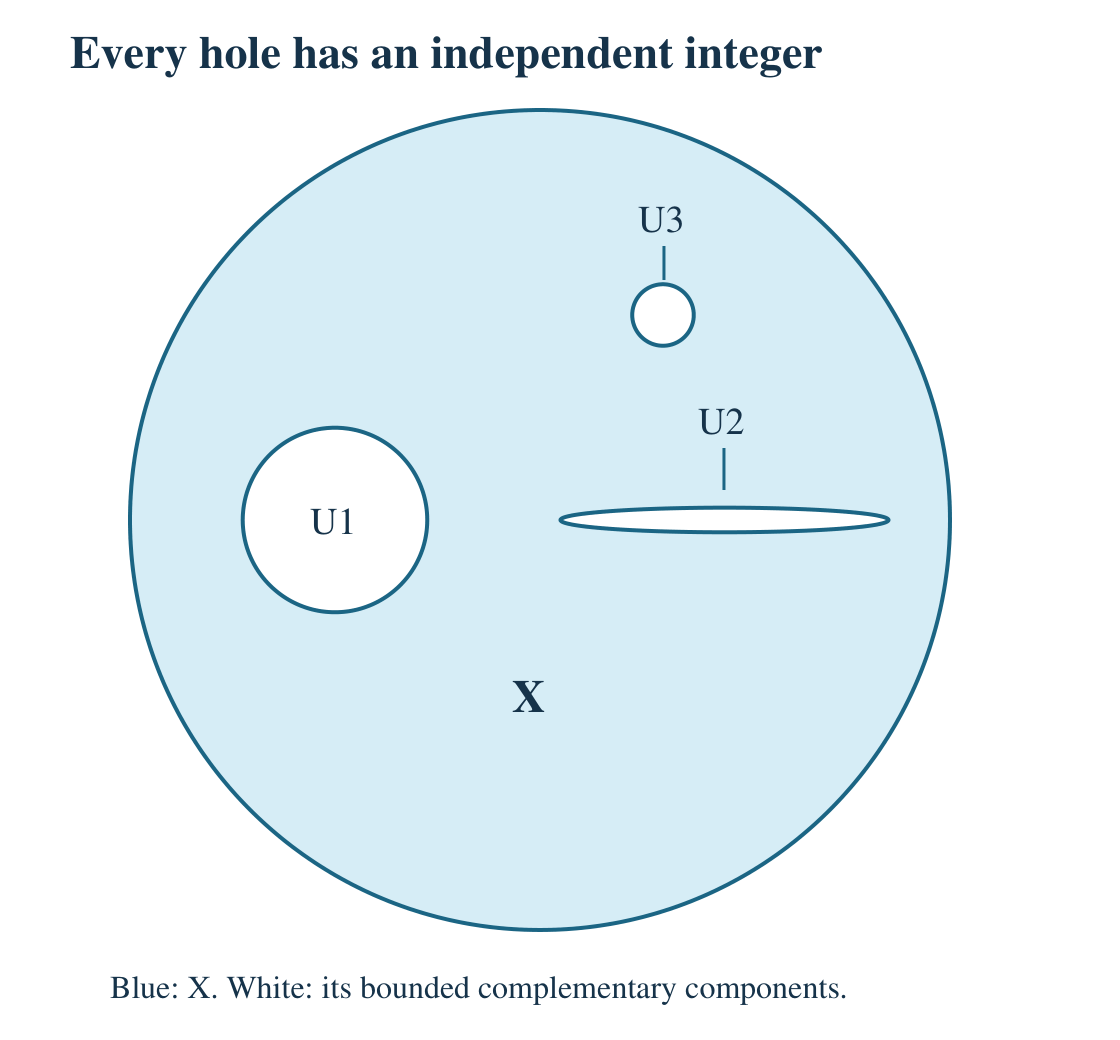
\includegraphics[keepaspectratio,alt={The compact set X is a closed disk with three open holes: a larger disk, a long thin ellipse, and a smaller disk.}]{assets/planar-holes.png}}

\emph{Figure 1. An exact example for Theorem 5.3: remove from the closed
disk of radius \(2\) the open disk centered at \((-1,0)\) of radius
\(9/20\), the open ellipse centered at \((9/10,0)\) with semiaxes
\(4/5\) and \(3/50\), and the open disk centered at \((3/5,1)\) of
radius \(3/20\). The long thin hole has a smaller area than the larger
disk.}

The quantitative bounds of Lemma 5.2 in this example are:

{\def\LTcaptype{none} % do not increment counter
\begin{longtable}[]{@{}llll@{}}
\toprule\noalign{}
Hole & Area & Bound \(4a(U_j)/\pi\) & Chosen index \\
\midrule\noalign{}
\endhead
\bottomrule\noalign{}
\endlastfoot
\(U_1\) & \(81\pi/400\) & \(81/100\) & \(-2\) \\
\(U_2\) & \(6\pi/125\) & \(24/125\) & \(3\) \\
\(U_3\) & \(9\pi/400\) & \(9/100\) & \(0\) \\
\end{longtable}
}

For the chosen sequence, take two Bergman shifts on \(U_1\), three
adjoint shifts on the reflection of \(U_2\), and no hole summand for
\(U_3\). Add a diagonal normal operator with essential spectrum \(X\).
This last summand supplies essential spectrum on all of \(X\), while the
indices come from the hole summands.

\subsection{6. Absorption on a Hilbert
space}\label{absorption-on-a-hilbert-space}

An extension \(\tau\) is \textbf{absorbing} if
\(\tau\oplus\sigma\sim_s\tau\) for every split extension \(\sigma\). If
\(A\) is unital, it is \textbf{unital-absorbing} if this holds for every
split extension with a unital homomorphic lift. This is stronger than
representing the same stable class: here a single multiplier unitary
must implement the equivalence.

The proof needs a way to place a prescribed finite-dimensional positive
map far out in a Hilbert space. We develop that approximation first,
then turn it into an intertwiner and a unitary. The freely accessible
comparison account is {[}Blackadar, free corrected \emph{K-Theory},
15.12{]}. The compactness, compression and unitary constructions used
here are written out below.

\subsubsection{Lemma 6.1. Singular states can be approximated away from
finite-dimensional
subspaces}\label{lemma-6.1.-singular-states-can-be-approximated-away-from-finite-dimensional-subspaces}

Let \(D\subset\mathcal B(H)\) be a unital C*-algebra on an
infinite-dimensional Hilbert space. A state \(\omega\) that vanishes on
\(D\cap\mathcal K(H)\) can be approximated, on any finite subset of
\(D\), by a vector state of a unit vector orthogonal to any prescribed
finite-dimensional subspace of \(H\).

\textbf{Proof.} Replace \(D\) by \(D+\mathcal K(H)\), extending
\(\omega\) to be zero on the added compact ideal. This extension exists
as a state because the map

\[
D/(D\cap\mathcal K(H))\longrightarrow
(D+\mathcal K(H))/\mathcal K(H)
\]

is an isomorphism. It is an injective, surjective C*-homomorphism, hence
isometric. We may thus assume that \(D\) contains the compact operators.

For each finite-dimensional \(F\subset H\), let \(C_F\) be the weak-star
closure in the state space of the vector states of unit vectors in
\(F^\perp\). Put \(C=\bigcap_F C_F\). The sets are compact and have the
finite intersection property, because passing to the sum of finitely
many subspaces gives a smaller nonempty set. Thus \(C\) is nonempty and
compact. Every state in \(C\) vanishes on compacts: a compact operator
can be approximated in norm by an operator supported on a
finite-dimensional subspace, and the latter has expectation zero on its
orthogonal complement.

The set \(C\) is convex. To approximate a convex combination
\(t\rho+(1-t)\eta\), with \(\rho,\eta\in C\), on operators
\(a_1,\ldots,a_m\), choose a unit vector \(\xi\in F^\perp\)
approximating \(\rho\). Then choose a unit vector \(\zeta\)
approximating \(\eta\) and orthogonal to

\[
F+\operatorname{span}\{\xi,a_i\xi,a_i^*\xi:1\leq i\leq m\}.
\]

The vector \(\sqrt t\,\xi+\sqrt{1-t}\,\zeta\) has norm one, lies in
\(F^\perp\), and its cross terms vanish on every \(a_i\). Its state
therefore approximates the desired convex combination. Since \(F\), the
finite set and the tolerance were arbitrary, the combination lies in
\(C\).

For \(a=a^*\in D\), let \(m\) be the largest point of the spectrum of
\(q(a)\). We claim

\[
\max_{\rho\in C}\rho(a)=m.
\]

For the upper bound, \((a-(m+\varepsilon)1)_+\) is compact by functional
calculus. Outside a sufficiently large finite-dimensional subspace, its
expectations are smaller than \(\varepsilon\), so states in \(C\) have
expectation at most \(m+2\varepsilon\). Let \(\varepsilon\to0\).

For the lower bound, on the orthogonal complement of any
finite-dimensional subspace the supremum of the expectations of \(a\) is
at least \(m\). Otherwise the compression there would be bounded above
by a scalar \(c<m\). It differs from \(a\) by a finite-rank operator, so
it would imply \(q(a)\leq c1\), contradicting the definition of \(m\).
Choose vectors in these complements with expectations tending to \(m\),
and take a weak-star cluster point of their states. It lies in \(C\) and
has expectation at least \(m\).

If \(\omega\notin C\), Hahn--Banach separation of the compact convex set
\(C\) gives a self-adjoint \(a\) with
\(\omega(a)>\max_{\rho\in C}\rho(a)\), after changing its sign if
necessary. But \(\omega\) is a state of \(D/\mathcal K(H)\), so
\(\omega(a)\leq m\), contradicting the claim. Hence \(\omega\in C\). Its
membership in every \(C_F\) is exactly the required approximation
statement. \(\square\)

\subsubsection{Lemma 6.2. Finite matrix
compressions}\label{lemma-6.2.-finite-matrix-compressions}

Let \(D\subset\mathcal B(H)\) be unital, and let
\(\gamma:D\to M_n(\mathbb C)\) be a completely positive contraction
vanishing on \(D\cap\mathcal K(H)\). Given a finite set and a tolerance,
there is a contraction \(W:\mathbb C^n\to H\), with range orthogonal to
any prescribed finite-dimensional subspace, such that \(W^*aW\)
approximates \(\gamma(a)\) on that set. We may require
\(W^*W=\gamma(1)\). In particular \(W\) is an isometry if \(\gamma\) is
unital.

\textbf{Proof.} If \(s=\operatorname{Tr}\gamma(1)=0\), positivity forces
\(\gamma=0\), and take \(W=0\). Otherwise

\[
\Omega([a_{ij}])=s^{-1}\sum_{i,j}
\langle e_i,\gamma(a_{ij})e_j\rangle
\]

is a state on \(M_n(D)\). Positivity follows by applying the positive
matrix \(\gamma^{(n)}([a_{ij}])\) to the vector \((e_1,\ldots,e_n)\),
and the normalization is \(\Omega(1)=1\). It vanishes on compact
operators in \(M_n(D)\).

Apply Lemma 6.1 to the matrix-unit multiples of the finite set,
including \(1\), and exclude the \(n\)-fold sum of the prescribed
subspace. A unit vector \((\xi_1,\ldots,\xi_n)\in H^n\) then has matrix
expectations as close as required to those of \(\Omega\). Setting
\(W_0 e_j=\sqrt s\,\xi_j\) gives \(W_0^*aW_0\) as close as required to
\(\gamma(a)\), entry by entry and hence in operator norm.

If \(\gamma(1)\) is invertible, replace \(W_0\) by

\[
W=W_0(W_0^*W_0)^{-1/2}\gamma(1)^{1/2}.
\]

As the approximations improve, the correction tends to the identity, so
the matrix approximations persist and \(W^*W=\gamma(1)\). If
\(\gamma(1)\) has a kernel, all \(\gamma(a)\) vanish on that kernel and
have range in its orthogonal complement. For self-adjoint \(a\), this
follows from \(-\|a\|\gamma(1)\leq\gamma(a)\leq\|a\|\gamma(1)\); the
general case follows by linear decomposition. Apply the invertible
argument on the finite-dimensional support of \(\gamma(1)\), then extend
by zero. In either case the correction preserves the range, and
\(\|W\|^2=\|\gamma(1)\|\leq1\). \(\square\)

We also need a positive partition of the identity whose pieces almost
commute with prescribed operators. The following form works on Hilbert
modules as well as Hilbert spaces.

\subsubsection{Lemma 6.3. A quasicentral compact
partition}\label{lemma-6.3.-a-quasicentral-compact-partition}

Let \(J\) be a \(\sigma\)-unital C*-algebra, and let \(S\subset M(J)\)
be a separable set. There are positive contractions \(r_j\in J\) with
\(\sum_j r_j^2=1\) strictly, such that \(\sum_j\|[r_j,a]\|<\infty\) for
a dense set of \(a\in S\). Given a finite subset of \(S\) and
\(\varepsilon>0\), this sum can be made smaller than \(\varepsilon\) on
that subset. The map

\[
\Lambda(a)=\sum_jr_jar_j
\]

is completely positive and unital on \(M(J)\), and \(\Lambda(a)-a\in J\)
for every \(a\in S\). It is within \(\varepsilon\) of \(a\) on the
prescribed finite set.

\textbf{Proof.} Choose a positive contraction \(h\in J\) such that
suitable continuous cutoffs \(e_m=f_m(h)\) form an approximate identity.
Here one may take \(h=\sum_n2^{-n}b_n\), where \((b_n)\) is a positive
contractive countable approximate identity. The inequality
\(b_n\leq2^nh\) implies

\[
\|b_n^{1/2}(1-h(h+\delta)^{-1})\|^2
\leq 2^n\delta/4.
\]

It follows first for \(b_nx\), then for every \(x\in J\), that
\(h(h+\delta)^{-1}x\to x\), on both sides. Cutoffs that vanish near
zero, equal one above a decreasing threshold, and increase to one on
\((0,1]\) have the same approximate-identity property. Choose the
thresholds so that sufficiently later cutoffs are identically one on the
support of each earlier cutoff.

Let \(E=C^*(J,S,1)\subset M(J)\). For each \(a\in E\), the commutators
\([e_m,a]\) tend weakly to zero in \(J\). To check all the functionals
involved, extend a functional on \(J\) to \(E\) by Hahn--Banach. Express
it as a linear combination of positive functionals and use their GNS
representations. In any representation, \(e_m\) tends strongly to the
projection onto \(\overline{JH}\). This subspace is reducing for \(E\),
because \(J\) is an ideal, so its projection commutes with \(E\). Every
positive functional is a vector functional in its GNS representation.
Its values on the commutators therefore tend to zero, and so do those of
the original functional.

For finitely many \(a_i\), apply Hahn--Banach to the convex hull of a
tail of the tuples \(([e_m,a_i])_i\). Zero is in its norm closure;
otherwise a separating functional would contradict weak convergence to
zero. Thus a finite convex combination of arbitrarily late \(e_m\)'s has
arbitrarily small commutators with all these \(a_i\).

Build \(u_n\in J\) by these convex combinations. Require
\(u_nu_{n-1}=u_{n-1}\), which is possible by using cutoffs beyond the
support of all terms in \(u_{n-1}\), and require the minimum cutoff
index to tend to infinity. Then \(0\leq u_{n-1}\leq u_n\leq1\), and
\((u_n)\) is an approximate identity. Put \(u_0=0\) and
\(r_n=(u_n-u_{n-1})^{1/2}\).

The commutators of the square roots can be made summable. Explicitly,
uniformly approximate \(t^{1/2}\) on \([0,1]\) by a polynomial \(p\).
For \(\|a\|\leq1\),

\[
\|[c^{1/2},a]\|
\leq2\|t^{1/2}-p(t)\|_\infty
+C_p\|[c,a]\|,\qquad0\leq c\leq1,
\]

where \(C_p\) is the sum of the absolute coefficients weighted by their
degrees. Take increasing finite sets \(F_n\), containing the initially
prescribed set, with dense union in the normalized operators under
consideration. Choose the commutators of \(u_n\) on \(F_{n+1}\) small
enough for both the \(n\)-th and \((n+1)\)-st square-root tolerances.
The preceding estimate then gives

\[
\|[r_n,a]\|<\varepsilon2^{-n}
\quad(a\in F_n).
\]

For any \(a\) in their union the tail is summable; on the initially
prescribed set the whole sum is less than \(\varepsilon\). Also
\(\sum_{n\leq N}r_n^2=u_N\to1\) strictly.

The column \(x\mapsto(r_nx)_n\) is an adjointable isometry from \(J\),
or from the standard Hilbert module when \(J\) is its compact algebra,
into the countable direct sum. Compression of the diagonal
representation \(a\mapsto\operatorname{diag}(a,a,\ldots)\) gives the
unital completely positive map \(\Lambda\). The finite sums converge
strictly, by norm convergence of the column tails on every vector and
the same argument for adjoints. Finally,

\[
\Lambda(a)-a=\sum_nr_n[a,r_n].
\]

For the dense set this is a norm-convergent series of elements of \(J\),
with the asserted finite-set bound. Contractivity of \(\Lambda\) extends
the ideal-membership assertion to every \(a\in S\). \(\square\)

For \(J=\mathcal K(L)\), the cutoffs of \(h\) are finite rank. Hence
every \(r_n\) in the preceding construction is finite rank. Write
\(L_n=\operatorname{ran}r_n\), and let \(p_n\) project onto \(L_n\). The
isometry \(R:L\to\bigoplus L_n\), \(R\xi=(r_n\xi)_n\), satisfies

\[
\Lambda(a)=R^*\left(\bigoplus_np_na|_{L_n}\right)R.
\]

\subsubsection{Lemma 6.4. A representation can be embedded modulo
compact
errors}\label{lemma-6.4.-a-representation-can-be-embedded-modulo-compact-errors}

Let \(D\subset\mathcal B(H)\) be separable and unital, and let
\(\rho:D\to\mathcal B(L)\) be a unital representation on a separable
Hilbert space, vanishing on \(D\cap\mathcal K(H)\). Given a finite set
and \(\varepsilon>0\), there is an isometry \(V:L\to H\) such that

\[
aV-V\rho(a)\in\mathcal K(L,H)\quad(a\in D),
\]

and these errors have norm smaller than \(\varepsilon\) on the finite
set.

\textbf{Proof.} First consider a unital completely positive map
\(\varphi:D\to\mathcal B(L)\) that kills the same compact ideal. Apply
Lemma 6.3 to \(\varphi(D)\), using its generated separable algebra, to
make \(\Lambda\varphi(a)-\varphi(a)\) compact for all \(a\), and small
on a chosen finite set. The displayed factorization of \(\Lambda\)
writes it as an isometric compression of the block map

\[
\gamma(a)=\bigoplus_n\gamma_n(a),\qquad
\gamma_n(a)=p_n\varphi(a)|_{L_n}.
\]

Each \(\gamma_n\) is a unital finite-matrix completely positive map and
kills the compact ideal in \(D\).

Choose increasing finite sets \(F_n\subset D\), closed under adjoints,
containing \(1\) and the initial finite set, with dense union in the
unit ball. Lemma 6.2 supplies isometries \(W_n:L_n\to H\) whose
compressions approximate \(\gamma_n\) to tolerance \(\delta2^{-n}\) on
\(F_n\). Inductively require their ranges to be orthogonal to

\[
\operatorname{span}\{aW_iL_i:a\in F_n, i<n\}.
\]

This is finite dimensional. In particular their ranges are mutually
orthogonal. Thus \(W=\bigoplus W_n:\bigoplus L_n\to H\) is an isometry.

For \(a\in F_m\), every off-diagonal block \(W_j^*aW_i\) vanishes
whenever \(j>i\) and \(j\geq m\); adjoint-closure gives the transposed
assertion. The remaining off-diagonal blocks involve only finitely many
finite-dimensional spaces. On the diagonal, the tail errors tend to
zero. Therefore \(W^*aW-\gamma(a)\) is compact. For the initial finite
set all off-diagonal blocks vanish and the error norm is at most
\(\delta\). Density and boundedness extend compactness to all
\(a\in D\).

Set \(V=WR\). Then \(V\) is an isometry, and \(V^*aV-\varphi(a)\) is
compact for all \(a\) and as small as desired on any chosen finite set.

Now take \(\varphi=\rho\). With \(e(a)=V^*aV-\rho(a)\), direct expansion
gives

\[
(aV-V\rho(a))^*(aV-V\rho(a))
=e(a^*a)-e(a^*)\rho(a)-\rho(a^*)e(a).
\]

The right side is compact. An operator whose square modulus is compact
is compact: cut off the spectral subspaces of that square above a
positive threshold and let the threshold decrease to zero. More
explicitly, if \(\|e(a)\|,\|e(a^*)\|,\|e(a^*a)\|<\eta\), then

\[
\|aV-V\rho(a)\|^2\leq(1+2\|a\|)\eta.
\]

Enlarge the finite approximation set by \(a^*,a^*a\), and choose
\(\eta<\varepsilon^2/(1+2\max_{a\in F}\|a\|)\). This proves the required
norm estimate as well as compactness. \(\square\)

\subsubsection{Theorem 6.5. Voiculescu
absorption}\label{theorem-6.5.-voiculescu-absorption}

Every essential nonunital extension of a separable \(A\) by
\(\mathcal K\) is absorbing. For separable unital \(A\), every essential
unital extension is unital-absorbing.

\textbf{Proof.} We first turn Lemma 6.4 into unitary absorption. Write
\(\rho^\infty\) for a countably infinite sum of a representation
\(\rho\) as in that lemma. Choose an isometry \(V:L^\infty\to H\) with
compact intertwining errors. Put \(P=VV^*\), \(H_0=(1-P)H\), and
\(\psi(a)=(1-P)a|_{H_0}\). The map

\[
J:H_0\oplus L^\infty\longrightarrow H,\qquad
J(x,\eta)=x+V\eta
\]

is unitary. Its error in intertwining \(a\) with
\(\psi(a)\oplus\rho^\infty(a)\) is compact: on \(L^\infty\) it is
\(aV-V\rho^\infty(a)\), and on \(H_0\) it is \(Pa|_{H_0}\), whose
adjoint is controlled by the error for \(a^*\). Thus conjugation by
\(J\) identifies these two operator-valued maps modulo compacts.

Let \(S:L^\infty\oplus L\to L^\infty\) be the reindexing unitary, so
\(S(\rho^\infty(a)\oplus\rho(a))S^*=\rho^\infty(a)\). Then

\[
U=J(1_{H_0}\oplus S)(J^*\oplus1_L):H\oplus L\longrightarrow H
\]

is an actual unitary. Substituting the preceding compact intertwining
equation for \(J\) on the two sides gives
\(U(a\oplus\rho(a))U^*-a\in\mathcal K(H)\). This uses a single isometry
with compact errors for the infinite representation, rather than an
uncontrolled sum of compact errors from separate isometries. On a fixed
finite set, apply Lemma 6.4 also to adjoints, with error less than
\(\delta\). Each of the two columns of the error for \(J\) then has norm
less than \(\delta\), and the final error for \(U\) has norm at most
\(4\delta\). Taking \(\delta<\varepsilon/4\) proves the finite-set
approximation assertion.

For the unital assertion, realize the essential extension as a concrete
algebra \(E\subset\mathcal B(H)\) containing \(\mathcal K(H)\). The
multiplier projection is injective by the first lesson, and
\(E/\mathcal K(H)=A\). The algebra \(E\) is separable: lift a countable
generating set of \(A\) and add countably many matrix units for
\(\mathcal K(H)\). A unital split lift \(\sigma:A\to\mathcal B(L)\)
gives the unital representation \(\rho=\sigma\circ p\) of \(E\), killing
its compact ideal. The preceding unitary therefore conjugates the Busby
map of \(\tau\oplus\sigma\) to that of \(\tau\).

For a nonunital essential extension, adjoin the ambient identity to
\(E\). Its quotient is the adjoined-unit algebra \(A^+\). Indeed
\(1\notin\tau(A)\): if \(A\) is nonunital, injectivity of \(\tau\) would
otherwise produce a unit in \(A\); if \(A\) is unital, the stipulated
nonunitality gives \(\tau(1_A)\ne1\), and \(\tau(A)\) has that proper
support. Hence the extension of \(A^+\) remains essential and is unital.
Every split lift \(\sigma:A\to\mathcal B(L)\), including a degenerate
one, extends to the unital lift
\(\sigma^+(a+\lambda)=\sigma(a)+\lambda1\). Apply the unital assertion
and restrict to \(A\). This gives absorption of every split extension.
\(\square\)

An absorbing extension may therefore be described without adding an
unspecified split summand in its equivalence relation. If two absorbing
extensions have the same stable class, their stable equivalence and the
absorption of its split summands give a strong equivalence between the
original extensions. Conversely strong equivalence always gives the same
stable class.

\subsection{7. Kasparov absorption with a coefficient
algebra}\label{kasparov-absorption-with-a-coefficient-algebra}

For a general ideal \(B\otimes\mathcal K\), essentiality alone does not
ensure absorption. The correct theorem supplies a particular absorbing
split extension, obtained by tensoring an essential Hilbert-space
representation with the multiplier identity of \(B\). Nuclearity is the
condition that lets us imitate finite matrix compressions locally on the
module.

Here nuclearity is used in the finite-matrix formulation (3.0), just as
in Section 3. Lemma 3.0e proves its preservation by unitization, without
a separability assumption. The proof below also checks its preservation
by \(B\otimes\mathcal K\). Theorem 3.0 proves the equivalence with
tensor-norm nuclearity at the original arbitrary-algebra generality.

\subsubsection{Lemma 7.1. Local finite-matrix
factorizations}\label{lemma-7.1.-local-finite-matrix-factorizations}

Let \(C\) be unital and separable, \(B\) be \(\sigma\)-unital,
\(\sigma:C\to\mathcal L(H_B)\) be a unital representation, and
\(r\in\mathcal K(H_B)\) be a positive contraction. If either \(C\) or
\(B\) is nuclear, the map

\[
\varphi_r(a)=r\sigma(a)r:C\longrightarrow\mathcal K(H_B)
\]

is approximated in point norm by completely positive contractions
through matrix algebras.

\textbf{Proof.} If \(C\) is nuclear, compose its finite-matrix
approximations with \(\varphi_r\). If \(B\) is nuclear, the algebra
\(\mathcal K(H_B)=B\otimes\mathcal K\) has the same approximation
property. To check this last assertion, first compress a finite set to a
large finite coordinate corner \(M_m(B)\); the compression and the
inclusion of that corner are completely positive contractions. Apply a
finite-matrix approximation of \(B\) simultaneously to its finitely many
entries. Its \(m\)-fold amplification and the corner inclusion give an
approximation of the original finite set through
\(M_m(M_n(\mathbb C))\). Matrix amplification is contractive for these
completely positive contractions. This proves the assertion for
\(B\otimes\mathcal K\). Compose its approximations with \(\varphi_r\).
\(\square\)

\subsubsection{Lemma 7.2. Finite coefficient
coordinates}\label{lemma-7.2.-finite-coefficient-coordinates}

Let \(\beta:M_n(\mathbb C)\to\mathcal K(H_B)\) be a completely positive
contraction. On any finite set of matrices it can be approximated by a
map

\[
b\longmapsto V^*(b\otimes1_r\otimes1_{M(B)})V,
\qquad V:H_B\longrightarrow\mathbb C^{nr}\otimes B,
\]

where \(r\) is finite and \(V\) is compact, adjointable and contractive.

\textbf{Proof.} Let \(P_m\) be the projection onto the first \(m\)
standard coordinates of \(H_B\). The definition of module compacts gives
\(P_m kP_m\to k\) in norm for every \(k\in\mathcal K(H_B)\). Thus
\(\beta_m(b)=P_m\beta(b)P_m\), regarded as a map into \(M_m(B)\),
approximates \(\beta\) on the finite set. This is still a completely
positive contraction.

The Choi matrix \(C=[\beta_m(e_{ij})]_{i,j=1}^n\in M_n(M_m(B))\) is
positive. Indeed \([e_{ij}]\) is positive in \(M_n(M_n(\mathbb C))\),
being the product of the column \((e_{i1})_i\) and its adjoint, and
complete positivity preserves this matrix positivity. Write \(C=R^*R\),
with \(R=C^{1/2}\). For each \(i\), let \(R_i:B^m\to B^{nm}\) be the
\(i\)-th block column of \(R\). Then \(R_i^*R_j=C_{ij}\).

Set \(r=nm\), let \(p_m:H_B\to B^m\) be coordinate restriction, and
define

\[
Vx=\sum_{i=1}^ne_i\otimes R_ip_mx.
\]

Its entries belong to \(B\), so it is a compact adjointable map between
these standard modules. Multiplication gives

\[
V^*(b\otimes1_r\otimes1)V
=p_m^*\beta_m(b)p_m=P_m\beta(b)P_m.
\]

Taking \(b=1\) gives \(V^*V=P_m\beta(1)P_m\leq1\), so \(V\) is
contractive. This proves the approximation statement. \(\square\)

\subsubsection{Lemma 7.3. An intertwiner for the tensor
representation}\label{lemma-7.3.-an-intertwiner-for-the-tensor-representation}

Let \(\pi:C\to\mathcal B(H)\) be a unital representation of a separable
unital algebra with \(\pi(C)\cap\mathcal K(H)=0\) and with \(\pi\)
faithful. Let \(B\) be \(\sigma\)-unital, and let
\(\Pi=\pi\otimes1_{M(B)}\) act on \(H\otimes B\cong H_B\). If either
\(C\) or \(B\) is nuclear, every unital representation
\(\sigma:C\to\mathcal L(H_B)\) admits an isometry \(W:H_B\to H_B\) such
that

\[
\Pi(a)W-W\sigma(a)\in\mathcal K(H_B)
\]

for all \(a\in C\). These errors can be arbitrarily small on any finite
set.

\textbf{Proof.} Apply Lemma 6.3 to \(J=\mathcal K(H_B)\) and
\(\sigma(C)\), obtaining compact positive \(r_j\) with \(\sum r_j^2=1\)
strictly and a localization \(\Lambda\sigma\) close to \(\sigma\) modulo
compacts. Choose increasing adjoint-closed finite sets \(F_j\subset C\),
containing \(1\) and the prescribed finite set, with dense union in the
unit ball. Choose a positive summable sequence \(\delta_j\), whose sum
is as small as needed.

By Lemma 7.1, factor the map \(a\mapsto r_j\sigma(a)r_j\), within
\(\delta_j/3\) on \(F_j\), as

\[
C\overset{\gamma_j}{\longrightarrow}M_{n_j}(\mathbb C)
\overset{\beta_j}{\longrightarrow}\mathcal K(H_B),
\]

with both maps completely positive and contractive. Lemma 7.2 gives a
finite \(r_j'\) and a compact contraction
\(V_j:H_B\to\mathbb C^{n_jr_j'}\otimes B\) such that
\(V_j^*(b\otimes1_{r_j'}\otimes1)V_j\) approximates \(\beta_j(b)\)
within \(\delta_j/3\) on \(\gamma_j(F_j)\). Write
\(\widetilde\gamma_j(a)=\gamma_j(a)\otimes1_{r_j'}\).

Apply Lemma 6.2 to \(\widetilde\gamma_j\circ\pi^{-1}\) on \(\pi(C)\).
Its compact-vanishing condition is automatic, since
\(\pi(C)\cap\mathcal K(H)=0\). Obtain a finite-dimensional-range
contraction \(T_j:\mathbb C^{n_jr_j'}\to H\) whose compressions
approximate \(\widetilde\gamma_j\) within \(\delta_j/3\) on \(F_j\).
Arrange its range, inductively, to be orthogonal to

\[
\operatorname{span}\{\pi(a)\operatorname{ran}T_i:
a\in F_j, i<j\}.
\]

Set \(Y_j=(T_j\otimes1_{M(B)})V_j:H_B\to H\otimes B\). These are compact
maps into mutually orthogonal Hilbert-coordinate submodules of the
original target module, and

\[
\|Y_j^*\Pi(a)Y_j-r_j\sigma(a)r_j\|<\delta_j
\quad(a\in F_j).
\]

In particular, with \(a=1\), the series

\[
h=\sum_jY_j^*Y_j
=1+\sum_j(Y_j^*Y_j-r_j^2)
\]

converges strictly, and \(h-1\) is a compact norm-convergent sum of norm
at most \(\sum\delta_j\). Choose that sum smaller than \(1/2\); then
\(h\) is positive and invertible.

The series \(Y=\sum_jY_j\) defines an adjointable map. Here are the
convergence checks. For \(x\in H_B\), orthogonality gives

\[
\left\|\sum_{j>N}Y_jx\right\|^2
=\left\|\left\langle x,\left(\sum_{j>N}Y_j^*Y_j\right)x\right\rangle\right\|\longrightarrow0,
\]

by strict convergence of the positive sums. If \(p_j\) projects onto the
finite-dimensional Hilbert-space range of \(T_j\), the \(p_j\)'s are
orthogonal, and \(\sum p_j\otimes1\) converges strongly on every module
vector. The finite partial-sum operators have uniformly bounded norm,
since their squared moduli are partial sums of the positive series
defining \(h\). Also \(Y_j^*=Y_j^*(p_j\otimes1)\). Hence, for \(M>N\),

\[
\left\|\sum_{j=N+1}^M Y_j^*y\right\|
\leq\sqrt{\|h\|}\,
\left\|\sum_{j=N+1}^M(p_j\otimes1)y\right\|\longrightarrow0.
\]

This proves convergence for the adjoint, giving \(Y^*y=\sum_jY_j^*y\).
We have \(Y^*Y=h\).

For \(a\in F_m\), all off-diagonal terms \(Y_j^*\Pi(a)Y_i\) with a
larger index at least \(m\) vanish. The remaining ones form a finite sum
of compact maps. The diagonal difference from \(\sum_j r_j\sigma(a)r_j\)
is a compact norm-convergent series: its tail norms are bounded by the
summable \(\delta_j\), and its finitely many earlier terms are compact.
Hence

\[
Y^*\Pi(a)Y-\sigma(a)\in\mathcal K(H_B).
\]

On the initial finite set there are no off-diagonal terms, and the norm
error is at most \(\sum\delta_j\) plus the localization error. Density
gives compactness for every \(a\in C\).

Normalize by putting \(W=Yh^{-1/2}\). Then \(W^*W=1\), and \(W-Y\) is
compact because \(h^{-1/2}-1\) is compact by functional calculus. Its
norm can be made arbitrarily small by reducing \(\sum\delta_j\). The
compression errors \(e(a)=W^*\Pi(a)W-\sigma(a)\) are therefore compact
and as small as desired on a finite set. The identity from Lemma 6.4,
with \(\Pi(a)\) replacing \(a\), gives

\[
(\Pi(a)W-W\sigma(a))^*(\Pi(a)W-W\sigma(a))
=e(a^*a)-e(a^*)\sigma(a)-\sigma(a^*)e(a).
\]

The map on the left is an endomorphism of the standard module. The
C*-identity in \(\mathcal L(H_B)/\mathcal K(H_B)\) therefore implies
that it is compact when its square modulus is compact. Enlarge the
initial finite set by \(a^*,a^*a\), and reduce the tolerances to obtain
the asserted norm estimates. \(\square\)

\subsubsection{Theorem 7.4. Kasparov's absorbing split
extension}\label{theorem-7.4.-kasparovs-absorbing-split-extension}

Let \(A\) be separable and \(B\) be \(\sigma\)-unital, and suppose
either \(A\) or \(B\) is nuclear. Let \(\pi:A\to\mathcal B(H)\) be a
homomorphic lift of an essential nonunital extension by
\(\mathcal K(H)\). Then the split extension of \(A\) by
\(B\otimes\mathcal K\) with lift

\[
\Pi(a)=\pi(a)\otimes1_{M(B)}
\]

is absorbing. If \(A\) is unital and the initial lift is unital and
essential modulo compacts, the tensor extension is unital-absorbing.

\textbf{Proof.} In the unital case, apply Lemma 7.3 to any unital split
lift \(\sigma:A\to\mathcal L(H_B)\), with its countably infinite direct
sum. Repeat the unitary construction in Theorem 6.5: the range
projection of the isometry \(W\) is adjointable, so
\(H_B=\operatorname{ran}W\oplus\operatorname{ran}(1-WW^*)\). The map
from the latter submodule plus the infinite sum of the domain to \(H_B\)
is unitary. Its errors are compact by the intertwining equations.
Reindexing the infinite copies absorbs one more copy of \(\sigma\), and
composing the two unitaries gives

\[
U(\Pi(a)\oplus\sigma(a))U^*-\Pi(a)
\in\mathcal K(H_B).
\]

This is exactly strong equivalence of the Busby maps.

In the nonunital case, pass to \(C=A^+\), with
\(\pi^+(a+\lambda)=\pi(a)+\lambda1\). This representation is faithful
and has no nonzero compact operator in its image: its Calkin map is
injective by the nonunital essentiality argument in Theorem 6.5. Extend
an arbitrary split lift \(\sigma\) to its unital \(\sigma^+\). If \(A\)
is nuclear, its unitization is nuclear; if \(B\) is nuclear, the
coefficient condition is unchanged. Apply the unital argument and
restrict to \(A\). \(\square\)

The theorem does not assert that every essential extension by
\(B\otimes\mathcal K\) absorbs split extensions. Its conclusion concerns
the tensor extension built from a faithful essential Hilbert-space lift.
This distinction is needed when using it to choose a zero representative
for \(\operatorname{Ext}(A,B)\).

Such zero representatives always exist under the theorem's hypotheses.
Choose a faithful representation of separable \(A\) on a separable
Hilbert space and repeat it infinitely. Every nonzero represented
element then has a nonzero action of fixed size on infinitely many
orthogonal vectors, so no nonzero image is compact. For the nonunital
absorbing version, append an infinite zero summand if necessary. This
gives the essential nonunital split lift required in Theorem 7.4; for
unital absorption use the unital infinite amplification. Both tensor
extensions are split and hence represent zero in their respective
stabilized semigroups.

More generally, if \(\sigma_0\) is an absorbing split extension, then
\(\tau\oplus\sigma_0\) is absorbing for every \(\tau\), by associativity
and absorption in the second summand. It has the same stable class as
\(\tau\). The map from strong classes of absorbing extensions to the
stabilized semigroup is consequently bijective: surjectivity follows
from this construction, and injectivity follows by absorbing the split
summands in a stable equivalence. The same argument works in the unital
variant with unital split summands.

\subsection{8. Why the planar indices
classify}\label{why-the-planar-indices-classify}

The construction in Section 5 supplied every integer sequence.
Injectivity involves more than local Fredholm theory. The extension
picture of odd KK and the universal coefficient theorem remain unproved
inputs. Their full statements and exact uses are given below. The planar
classification and the general compact-metric exact sequence therefore
remain conditional. Completing that obligation requires actual proofs of
the extension-class correspondence, its compatibility with the index
pairing, and the universal coefficient theorem, or a complete direct BDF
argument replacing them.

The missing extension-picture theorem would identify, for separable
\(A\), the invertible extension classes with \(KK^1(A,\mathbb C)\). Its
specified map sends a dilation \((\rho,P)\) of a semisplit extension to
the odd Fredholm module \((H,\rho,2P-1)\), with the usual extra summands
allowed. Under the asserted identification, its homomorphism on
\(K_1(A)\) evaluates a unitary by the Fredholm index of its compression
to \(PH\). \href{KT-KK-04.html}{The index pairing between K-theory and
K-homology}, Theorem 4.1, proves the compression's agreement with the
extension boundary. That compression calculation does not prove the full
class correspondence, its equivalence relations, or its agreement with
the Kasparov product; those remain missing.

The universal coefficient theorem says that, for a separable bootstrap
algebra \(A\) and separable \(B\), there is an exact sequence

\[
0\longrightarrow
\operatorname{Ext}^1_{\mathbb Z}(K_*(A),K_*(B))_{*+1}
\longrightarrow KK^*(A,B)
\overset{\gamma}{\longrightarrow}
\operatorname{Hom}_{\mathbb Z}(K_*(A),K_*(B))_*
\longrightarrow0.
\]

The subscripts specify the grading: \(\gamma\) has degree zero, while
the extension term shifts degree by one. The asserted map \(\gamma\) is
the action on operator K-theory through the Kasparov product. The
asserted sequence splits as a sequence of abelian groups, with no
natural choice of splitting. Membership of all separable commutative
C*-algebras in the bootstrap class and that splitting assertion are also
part of the missing theorem's scope. None of these assertions is being
treated as an available earlier proof.

\subsubsection{Lemma 8.1. The K-theory of a compact planar
set}\label{lemma-8.1.-the-k-theory-of-a-compact-planar-set}

For a compact \(X\subset\mathbb C\),

\[
K_0(C(X))\cong C(X,\mathbb Z),\qquad
K_1(C(X))\cong\bigoplus_j\mathbb Z,
\]

where \(j\) runs over the bounded components of the complement. The
second group has basis the classes of
\(u_{\lambda_j}(z)=(z-\lambda_j)/|z-\lambda_j|\). The first group is a
free abelian group.

\textbf{Proof.} Choose nested finite polygonal neighborhoods \(N_n\) of
\(X\), with \(X\subset\operatorname{int}N_n\),
\(N_{n+1}\subset\operatorname{int}N_n\), and \(\bigcap_nN_n=X\). One
construction uses the union of the closed squares of a sufficiently fine
grid that meet \(X\), together with all their neighboring squares.
Choose the next mesh small enough that this union lies inside the
preceding interior. Every component meets \(X\), and the distance of
\(N_n\) from \(X\) tends to zero.

Each \(N_n\) is a finite planar polyhedron that retracts onto a finite
graph. Triangulate its squares. As long as triangles remain, their union
has an exposed edge bordering the unbounded complementary region; an
edge at an extreme point of the finite union supplies one. Collapse its
incident triangle across that free edge, leaving the other two edges
fixed. This is a deformation retraction of the triangle together with
the rest of the complex onto the complex with the triangle and its free
edge removed. Repeating finitely many times leaves a graph. Components
made only of edges and vertices are already graphs.

For a finite graph, \(K_0\) is the group of integer ranks on its
components and \(K_1\) has one generator for each independent circuit.
Here are the K-theoretic inputs to this calculation: homotopy
invariance, the calculation \(K_0(C)=\mathbb Z\), \(K_1(C)=0\), the
circle calculation in operator K-theory, and Mayer--Vietoris. They are
proved in the programme's published operator K-theory lessons
\emph{Suspension, higher K-groups and the long exact sequence},
\emph{Toeplitz operators and the index theorem on the circle}, and
\emph{The six-term exact sequence and the exponential map}, Theorem 4.1.
Iterating the two-circle calculation in \emph{Topological K-theory of
spaces, pairs and vector bundles}, Exercise 12.3, gives a wedge of any
finite number of circles. Contracting a spanning tree gives the graph
calculation.

In a finite planar graph, the oriented boundaries of bounded faces form
a basis of the integral cycle group. Here are the integral relation
checks. A cycle is an integer flow on the oriented edges, with zero
total incoming minus outgoing coefficient at every vertex. It is a sum
of closed edge walks: follow a nonzero oriented edge until a vertex
repeats, subtract the resulting circuit with the least coefficient on
its edges, and repeat. The winding of these finitely many polygonal
walks defines an integer on each complementary face, zero on the
unbounded face. Across an oriented edge, its jump is exactly the
coefficient of that edge in the cycle, as is seen by a small transverse
passage past that edge in the argument integral. Consequently the cycle
is the sum of these face winding numbers times the oriented face
boundaries. For independence, a sum of face boundaries with zero edge
coefficients has equal coefficients on every pair of adjacent faces. The
dual adjacency graph is connected: a generic polygonal path to infinity
crosses finitely many edges and avoids all vertices. Thus all
coefficients equal the coefficient zero of the unbounded face. Filling
the triangulated faces inside \(N_n\) removes their boundary circuits.
Exactly the complementary bounded regions remain. The winding numbers
about a point in each remaining region therefore identify
\(K_1(C(N_n))\) with the free group on these regions. The scalar
unitaries \(u_\lambda\) have winding one about the region containing
\(\lambda\) and zero about the other regions, so they give that basis.

Restriction gives

\[
K_i(C(X))=\varinjlim_n K_i(C(N_n)).
\]

This is the continuity theorem in the published lesson \emph{Matrix
stability, stability and continuity of \(K_0\)}, together with its
suspension version for \(K_1\). Its hypotheses hold here: the direct
limit of the restriction system is \(C(X)\). The norms of restrictions
decrease to the norm on \(X\), since the neighborhoods are nested
compact sets with intersection \(X\). To check density explicitly, for
\(f\in C(X)\) choose a finite cover by disks with centers \(x_i\in X\)
and radius \(\delta/2\), where oscillations of \(f\) at distances
smaller than \(\delta\) are less than a given tolerance. Put
\(w_i(z)=(\delta-|z-x_i|)_+\). On a sufficiently small \(N_n\), the sum
of these weights is positive, and

\[
g(z)=\frac{\sum_iw_i(z)f(x_i)}{\sum_iw_i(z)}
\]

is continuous. On \(X\) it approximates \(f\) within the chosen
tolerance, since every nonzero weight has \(|z-x_i|<\delta\). This
proves density without assuming that a function on \(X\) has already
been extended to a neighborhood.

The limit of the rank groups is \(C(X,\mathbb Z)\). A continuous
integer-valued function on compact \(X\) has finitely many clopen level
sets. They have pairwise positive distances, so a sufficiently fine
neighborhood separates them and the function extends by constant ranks
on its components. Conversely ranks that agree on \(X\) agree on every
sufficiently small neighborhood: each of its components meets \(X\).
Thus the direct-limit rank map is an isomorphism.

For the \(K_1\) limit, a bounded complementary region of \(N_n\) lies in
one component of \(\mathbb C\setminus X\). Its \(u_\lambda\) maps to the
generator of that component if the component is bounded, and eventually
to zero if it is unbounded. The latter assertion follows by choosing a
path in \(\mathbb C\setminus X\) from \(\lambda\) to the exterior of a
disk containing all neighborhoods. Its compact part has positive
distance from \(X\), so a sufficiently small neighborhood misses it.

Every bounded component of \(\mathbb C\setminus X\) appears: choose a
point in it, which is eventually outside \(N_n\). Points in the same
component give the same generator in the limit, because a compact path
joining them is eventually disjoint from \(N_n\). Points in different
components never become joined in a neighborhood complement, since that
complement is contained in \(\mathbb C\setminus X\). These statements
also prove injectivity on a finite linear combination of generators: all
the finitely many path identifications needed for its cancellations
occur at one sufficiently late stage. The limit is therefore the
displayed direct sum, with the asserted basis.

Finally \(C(X,\mathbb Z)\) is free, not just torsion-free. There are
countably many clopen subsets of compact metric \(X\): each is a finite
union of members of a countable base, by compactness. Enumerate them and
let \(\mathcal P_n\) be the finite partitions obtained by successive
refinement. Then

\[
C(X,\mathbb Z)=\varinjlim_n\mathbb Z^{\mathcal P_n}.
\]

Refining one part into \(k\) nonempty parts sends its basis vector to
the sum of the \(k\) new basis vectors. That sum, together with all but
one of those new basis vectors, is an integral basis, so the inclusion
has a free complement. Successively choose these complements. The direct
limit is the direct sum of the initial finite free group and the
successive finite free complements, hence is free abelian. \(\square\)

\subsubsection{Theorem 8.2. Planar Brown--Douglas--Fillmore
classification}\label{theorem-8.2.-planar-browndouglasfillmore-classification}

For nonempty compact \(X\subset\mathbb C\), the map in Theorem 5.3 is an
isomorphism

\[
\operatorname{Ext}(C(X))\cong\prod_j\mathbb Z.
\]

\textbf{Conditional deduction; the proof obligation is still open.} The
algebra \(C(X)\) is separable and satisfies (3.0): approximate a finite
set of functions by evaluation at finitely many points, followed by a
nonnegative partition of unity subordinate to a cover on which those
functions have small oscillation. Evaluation is a homomorphism into
\(\mathbb C^n\); the reverse map is completely positive at every matrix
level because each value is a nonnegative weighted sum of positive
scalar matrices. Both maps are unital and contractive. Diagonal
inclusion into \(M_n\) and diagonal compression turn this into (3.0).
Thus all extension classes are invertible by Corollary 3.1. If the
missing extension-picture theorem is supplied, it gives

\[
\operatorname{Ext}(C(X))=KK^1(C(X),\mathbb C).
\]

The odd universal coefficient sequence becomes

\[
0\longrightarrow
\operatorname{Ext}^1_{\mathbb Z}(K_0(C(X)),\mathbb Z)
\longrightarrow KK^1(C(X),\mathbb C)
\longrightarrow\operatorname{Hom}(K_1(C(X)),\mathbb Z)
\longrightarrow0.
\]

The left group is zero because \(K_0(C(X))\) is free: every extension of
a free abelian group splits by choosing lifts of its basis elements.
Lemma 8.1 identifies the right group with the full product
\(\prod_j\mathbb Z\).

The resulting isomorphism would be precisely the index map. On a basis
unitary \(u_{\lambda_j}\), the asserted extension-picture and
index-pairing compatibility identifies the action of the extension class
with the index of its compressed lift, namely \(I_{\lambda_j}\). These
missing theorems would therefore imply injectivity. Surjectivity was
proved independently in Theorem 5.3. This records the remaining gap
rather than proving injectivity.

The freeness argument matters. Merely saying that a group is
torsion-free does not imply that its \(\operatorname{Ext}^1\) with
\(\mathbb Z\) vanishes. It is the explicit free decomposition of the
rank functions that closes the kernel calculation.

\subsubsection{Corollary 8.3. Classification of essentially normal
operators}\label{corollary-8.3.-classification-of-essentially-normal-operators}

Let \(T_1,T_2\) be essentially normal operators on an
infinite-dimensional separable Hilbert space, with the same essential
spectrum \(X\). They are unitarily equivalent modulo compacts if and
only if their Fredholm indices agree at every point of
\(\mathbb C\setminus X\).

An essentially normal \(T\) is a compact perturbation of a normal
operator if and only if all these indices vanish. If the complement of
\(X\) is connected, every such \(T\) is a compact perturbation of a
diagonal normal operator.

\textbf{Conditional deduction from the unresolved Theorem 8.2.} Their
functional-calculus Busby maps are essential and unital. If Theorem 8.2
has been proved, equal indices give equal stable extension classes. We
check that stabilization can then be removed even though its split
summands might initially be nonunital. Choose an evaluation character
\(\chi:C(X)\to\mathbb C\). In a stable equivalence between unital maps,
replace a split lift \(L_i\) by

\[
\widehat L_i(f)=L_i(f)+\chi(f)(1-L_i(1)).
\]

This is a unital homomorphism: the two summands have orthogonal support.
If the original sum has support projection \(p_i\) in the Calkin
algebra, the new sum is the original map plus \(\chi(f)(1-p_i)\). The
same multiplier unitary that conjugates the original sums conjugates
their support projections, and hence also these new unital sums. We have
obtained a stable equivalence using unital split summands. Theorem 6.5
absorbs those summands in each original extension. Consequently the
original Busby maps are strongly equivalent.

Apply that equality to the coordinate function \(z\). It says
\(UT_1U^*-T_2\) is compact. The converse follows from unitary and
compact-perturbation invariance of the Fredholm index.

For the normal-perturbation assertion, choose a diagonal operator \(D\)
whose entries are dense in \(X\), with infinite repetitions, as in
Theorem 5.3. Its Busby map is essential, unital and split, hence
represents zero. If \(T\)'s indices vanish, the preceding argument gives
\(UTU^*-D\) compact. Conversely a normal Fredholm operator has equal
kernel and cokernel dimensions, because
\(\ker(N-\lambda)=\ker(N^*-\bar\lambda)\); compact perturbations
preserve index. If the complement is connected, the only component is
unbounded and its index is zero. The diagonal conclusion then follows
from the same \(D\). \(\square\)

\subsubsection{The general compact metric
case}\label{the-general-compact-metric-case}

For any compact metric \(X\), not necessarily planar, the same
extension-picture and universal coefficient theorems give the natural
exact sequence

\[
0\longrightarrow
\operatorname{Ext}^1_{\mathbb Z}(K_0(C(X)),\mathbb Z)
\longrightarrow\operatorname{Ext}(C(X))
\longrightarrow\operatorname{Hom}(K_1(C(X)),\mathbb Z)
\longrightarrow0.
\]

The asserted last arrow pairs extensions with unitary K-theory classes
by their Fredholm index. Its proposed proof is the odd specialization of
the missing universal coefficient theorem, with \(B=\mathbb C\), and the
missing extension-picture identification. The asserted sequence is
natural in \(X\) and splits as abelian groups, with no natural choice of
splitting. These are preserved statements requiring proof, not
conclusions established in this lesson. Without the planar freeness
result its left-hand term need not vanish.

\subsection{9. Exercises}\label{exercises}

\textbf{Exercise 9.1 (basic).} Prove that the Toeplitz extension class
has infinite order. Construct a unitary lifting the sum of its Busby map
with the adjoint-shift map.

\textbf{Exercise 9.2 (intermediate).} Given two pairs of addition
isometries, construct the multiplier unitary identifying the sums. Check
that it also respects split lifts and stable equivalence.

\textbf{Exercise 9.3 (intermediate).} Starting from a completely
positive contractive lift, construct the complementary-corner inverse.
Prove that the off-diagonal dilation entries are compact, and explain
why a negative Busby map is not an inverse.

\textbf{Exercise 9.4 (advanced).} Let \(X=\{z:r\leq|z|\leq R\}\), with
\(0<r<R\). Compute \(\operatorname{Ext}(C(X))\) and give essentially
normal representatives for every class, with essential spectrum exactly
\(X\). Explain why a scaled shift by itself is insufficient for the last
requirement.

\subsection{10. Solutions}\label{solutions}

\textbf{Solution 9.1.} The index homomorphism sends the Toeplitz class
to \(-1\), so its \(n\)-fold sum has index \(-n\), which is nonzero for
\(n\ne0\). The block operator

\[
U=\begin{pmatrix}S&p_0\\0&S^*\end{pmatrix}
\]

is unitary by the multiplication in Theorem 4.2 and differs from
\(S\oplus S^*\) by rank one. The map \(f\mapsto f(U)\) therefore gives a
homomorphic lift of the sum, proving that the two classes are inverses.

\textbf{Solution 9.2.} For families \(s_i\) and \(t_i\), take
\(U=\sum_{i=1}^2t_is_i^*\). Orthogonality and completeness give
\(U^*U=UU^*=1\) and \(Us_i=t_i\). Conjugating the sum by \(q(U)\)
changes each \(s_i\) to \(t_i\). The same equality holds before taking
the quotient for homomorphic lifts, so split extensions stay split. If
stable equivalence is witnessed by split summands, conjugating the
corresponding sums does not change that property. Thus addition on the
quotient is independent of the choice.

\textbf{Solution 9.3.} Lemma 2.2 supplies a homomorphism
\(\Phi=[\Phi_{ij}]\) with \(\Phi_{11}=L\). Since \(qL\) is
multiplicative,

\[
q(\Phi_{21}(a)^*\Phi_{21}(a))
=q(L(a^*a)-L(a)^*L(a))=0.
\]

The C*-identity in the quotient gives \(q(\Phi_{21}(a))=0\). Taking
adjoints and replacing \(a\) by \(a^*\) gives the same for
\(\Phi_{12}\). Thus \(\tau'=q\Phi_{22}\) is multiplicative and
\(\tau\oplus\tau'\) has homomorphic lift \(\Phi\), after the standard
matrix identification. A negative map fails multiplicativity:
\((-\tau(a))(-\tau(b))=\tau(ab)\), whereas \(-\tau(ab)\) has the
opposite sign. The inverse comes from an orthogonal corner, not scalar
negation.

\textbf{Solution 9.4.} The complement has one bounded component, the
disk \(|z|<r\). The classification claim
\(\operatorname{Ext}(C(X))\cong\mathbb Z\), with coordinate
\(\operatorname{index}(T-\lambda)\) for \(|\lambda|<r\), follows
conditionally from Theorem 8.2; its injectivity is subject to the proof
gap stated there. The following representatives and index calculations
are unconditional. Choose a diagonal normal \(D\) with essential
spectrum \(X\). For \(k<0\), take

\[
T_k=(rS)^{\oplus|k|}\oplus D;
\]

for \(k>0\), take \(T_k=(rS^*)^{\oplus k}\oplus D\); and for \(k=0\),
take \(T_0=D\). They are essentially normal. Their essential spectra are
the union of the circle \(|z|=r\) with \(X\), hence exactly \(X\). Their
indices in the hole are respectively \(k\), and the index outside
\(|z|>R\) is zero. A scaled shift alone has essential spectrum only the
boundary circle, so it does not represent an essential extension of the
whole annulus without the normal summand.

\subsection{Internal proof dependencies and source
credit}\label{internal-proof-dependencies-and-source-credit}

The Busby correspondence and semisplitting criterion are proved in the
preceding lesson, Theorems 2.1 and 3.1. Its Lemmas 1.1--1.2 prove the
Hilbert-space Fredholm criterion and index properties. Lemma 2.0a here
proves strict KSGNS, Lemmas 2.1--2.2 prove stabilization and corner
dilation with arbitrary coefficients, Theorem 3.0 proves the nuclearity
equivalence, and Lemmas 3.0a--3.0e prove finite-matrix lifting,
quasicentral patching, exact lifting and the unitization approximation
argument. The existing Hilbert-module foundations linked at their exact
proof locations supply the module norm, completion, adjointable-operator
positivity and multiplier identification.

The compression pairing and its boundary interpretation are proved in
the linked index-pairing lesson. Theorem 3.0 proves the equivalence of
tensor nuclearity with (3.0), including the finite-dimensional duality,
tensor cone separation and nonunital passage. The extension-picture
correspondence, its product compatibility and the universal coefficient
theorem remain missing proof inputs in Section 8. Consequently Theorem
8.2, Corollary 8.3, the general compact-metric exact sequence and the
classification claim in Solution 9.4 remain conditional. Their full
statements and conditional deductions are given above. The realization
of all planar index sequences and both absorption constructions have
independent proofs above.

For Lemma 2.0b and Theorem 3.0, the earlier
\href{https://kokunoyumeto.github.io/open-math-courses/courses/foundations-of-von-neumann-algebras/c-star-algebras-continuous-functional-calculus-automatic-continuity-positive-cones.html}{C*-algebra
foundations} supply commutative Gelfand representation (Theorem 2.1),
automatic contractivity and isometry (Theorem 4.2 and Corollary 4.6),
continuous calculus and positive square roots (Theorems 5.1--5.3 and
Proposition 7.2), and contractive approximate identities (Theorem 11.4
and Corollary 11.5). The
\href{https://kokunoyumeto.github.io/open-math-courses/courses/foundations-of-von-neumann-algebras/hahn-banach-baire-and-the-basic-theorems-on-banach-spaces.html}{Hahn--Banach
lesson} proves the extensions in Theorems 2.1--2.2 and Corollary 2.3 and
the separation used here in Theorem 6.3 and Corollary 6.4. The actual
\href{https://kokunoyumeto.github.io/open-math-courses/courses/foundations-of-von-neumann-algebras/weak-topologies-tychonoff-banach-alaoglu-mazur-bipolars-krein-milman-and-eberlein-smulian.html}{weak-topology
lesson}, Theorem 1.2 and Theorem 3.1 with its Tychonoff proof, supplies
the weak-* dual and Banach--Alaoglu. Scalar GNS, faithful
representations, pure-state norming and every ordinary tensor assertion
needed here are proved in Lemma 2.0b itself.

\subsection{References}\label{references}

\begin{itemize}
\item
  B. Blackadar, \emph{K-Theory for Operator Algebras}, freely accessible
  author-corrected second-edition PDF. Sections 13.6--13.7 and
  15.6--15.8 concern stabilization, dilation, addition and
  semisplitting; Section 15.12 concerns absorption.
  \href{https://www.bruceblackadar.com/Mathematics/book6.pdf}{Free
  author version}.
\item
  B. Blackadar, \emph{Operator Algebras: Theory of C*-Algebras and von
  Neumann Algebras}, freely accessible author-revised version dated 8
  February 2017. II.9.3--II.9.5 develops states on tensors, minimality
  and matrix norm uniqueness, whose complete ordinary tensor argument is
  written in Lemma 2.0b; II.7.5.2 states strict KSGNS; IV.3.1.4--9
  states the nuclearity equivalence; IV.3.2.13--17 develops
  finite-matrix lifting and quasicentral patching.
  \href{https://www.bruceblackadar.com/Mathematics/Cycr.pdf}{Free
  revised author version}.
\item
  K. H. Han and V. I. Paulsen, \emph{An approximation theorem for
  nuclear operator systems}, Sections 2--3, especially Theorem 3.1 and
  Corollary 3.3. \href{https://arxiv.org/pdf/1009.2541}{Free arXiv
  version}. The finite-dimensional proof of Theorem 3.0 follows its
  method and supplies its supporting arguments.
\item
  A. S. Kavruk, V. I. Paulsen, I. G. Todorov and M. Tomforde,
  \emph{Tensor Products of Operator Systems}, Sections 5--6.
  \href{https://arxiv.org/pdf/0910.2210}{Free arXiv version}. Theorem
  3.0 uses its finite positive tensor cone and universal algebra; the
  required comparison is proved here by scalar GNS.
\end{itemize}

These freely readable source PDFs retain their authors' copyrights. The
CC0 notice above applies to this lesson's original text, not to the
referenced PDFs.

\end{document}
